\subsection{Promedio}

\begin{figure}[H]
\begin{center}
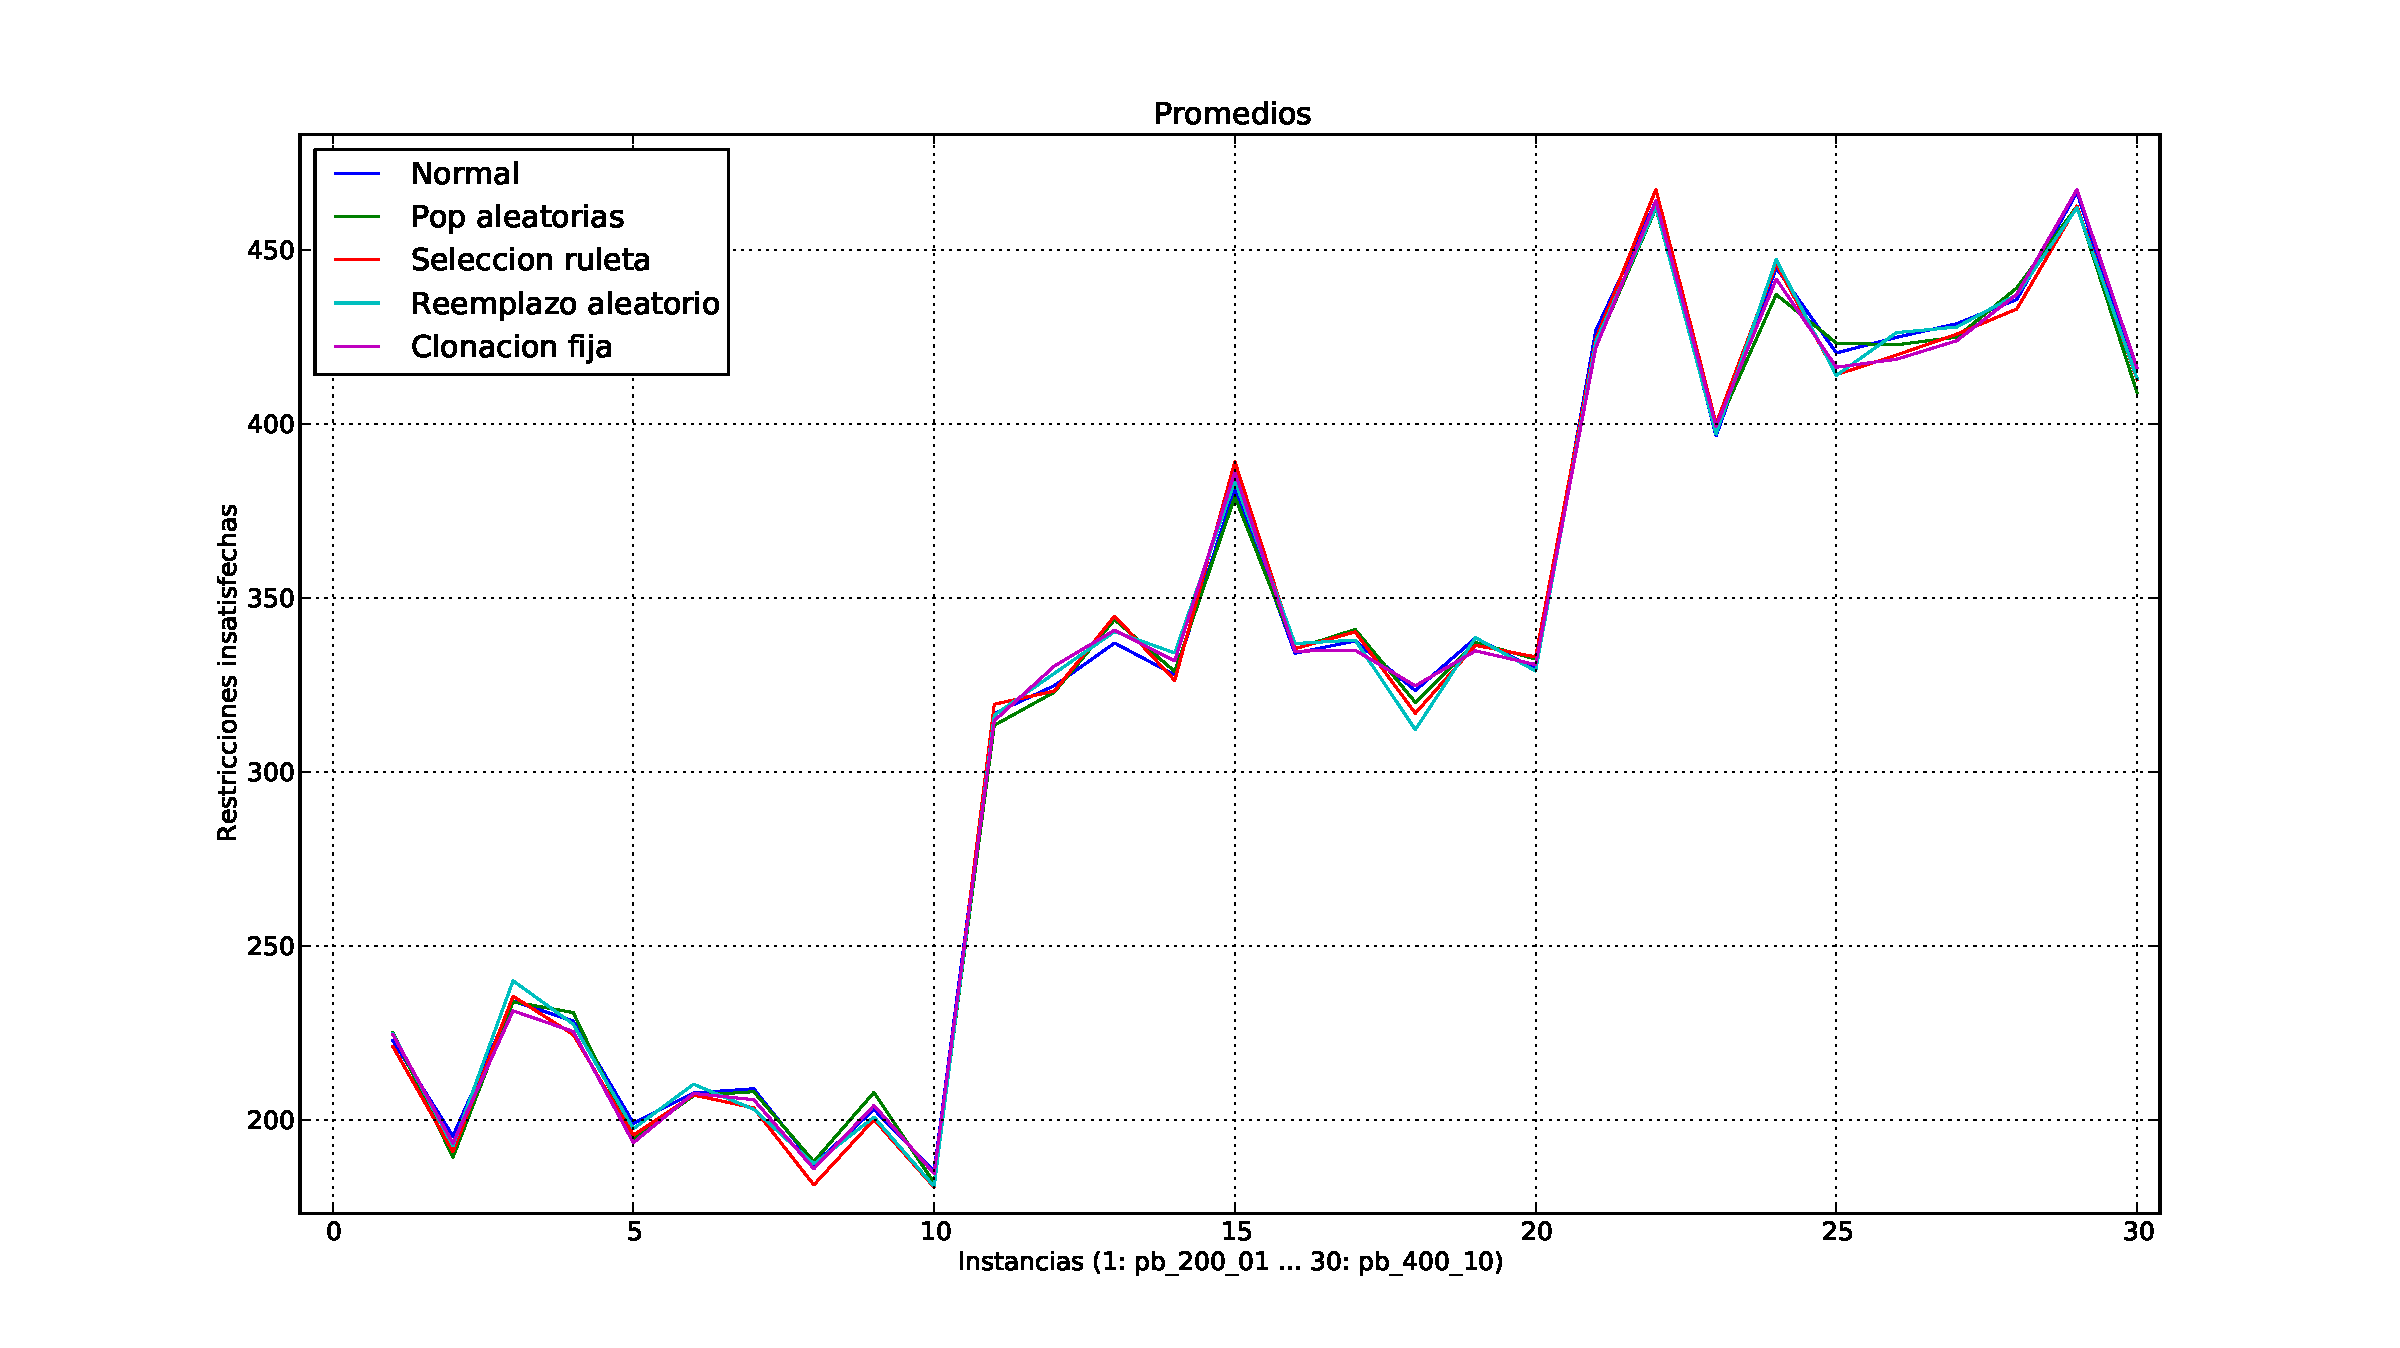
\includegraphics[width=0.95\textwidth]{img/promedio.pdf}
\end{center}
\caption{Promedio de valores para cada modificación}
\label{fig:promedio}
\end{figure}

\begin{figure}[H]
\begin{center}
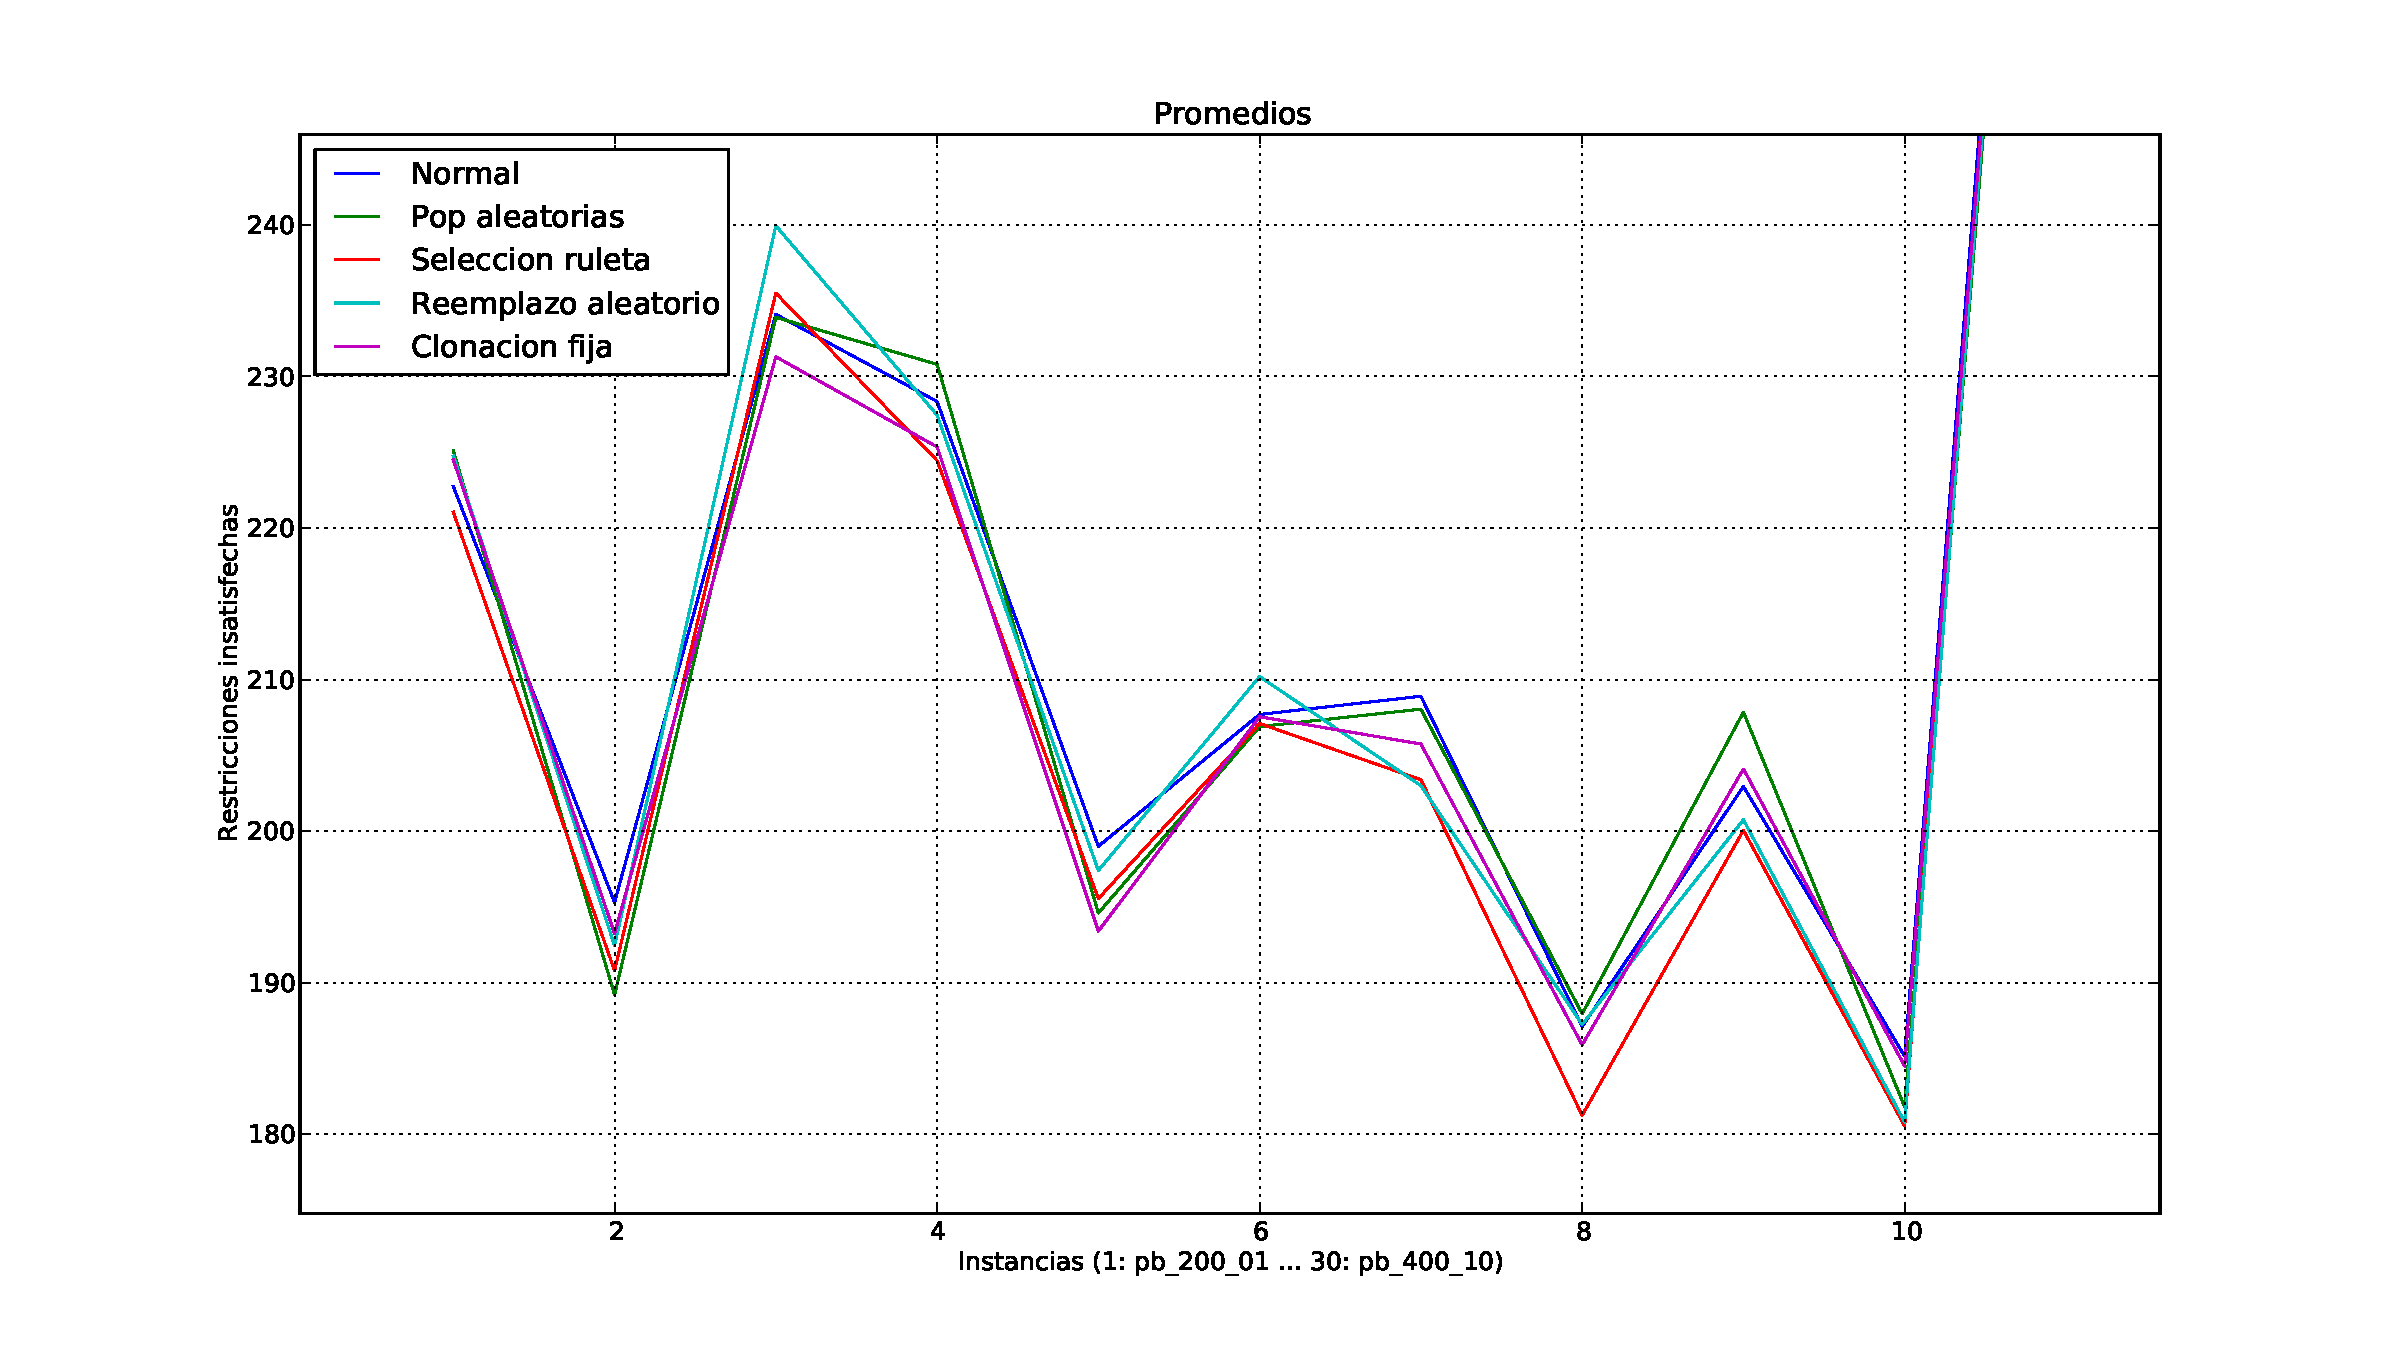
\includegraphics[width=0.95\textwidth]{img/promedio-zoom200.pdf}
\end{center}
\caption{Promedio de valores para cada modificación (Zoom a las instancias de 200)}
\label{fig:promedio200}
\end{figure}

\begin{figure}[H]
\begin{center}
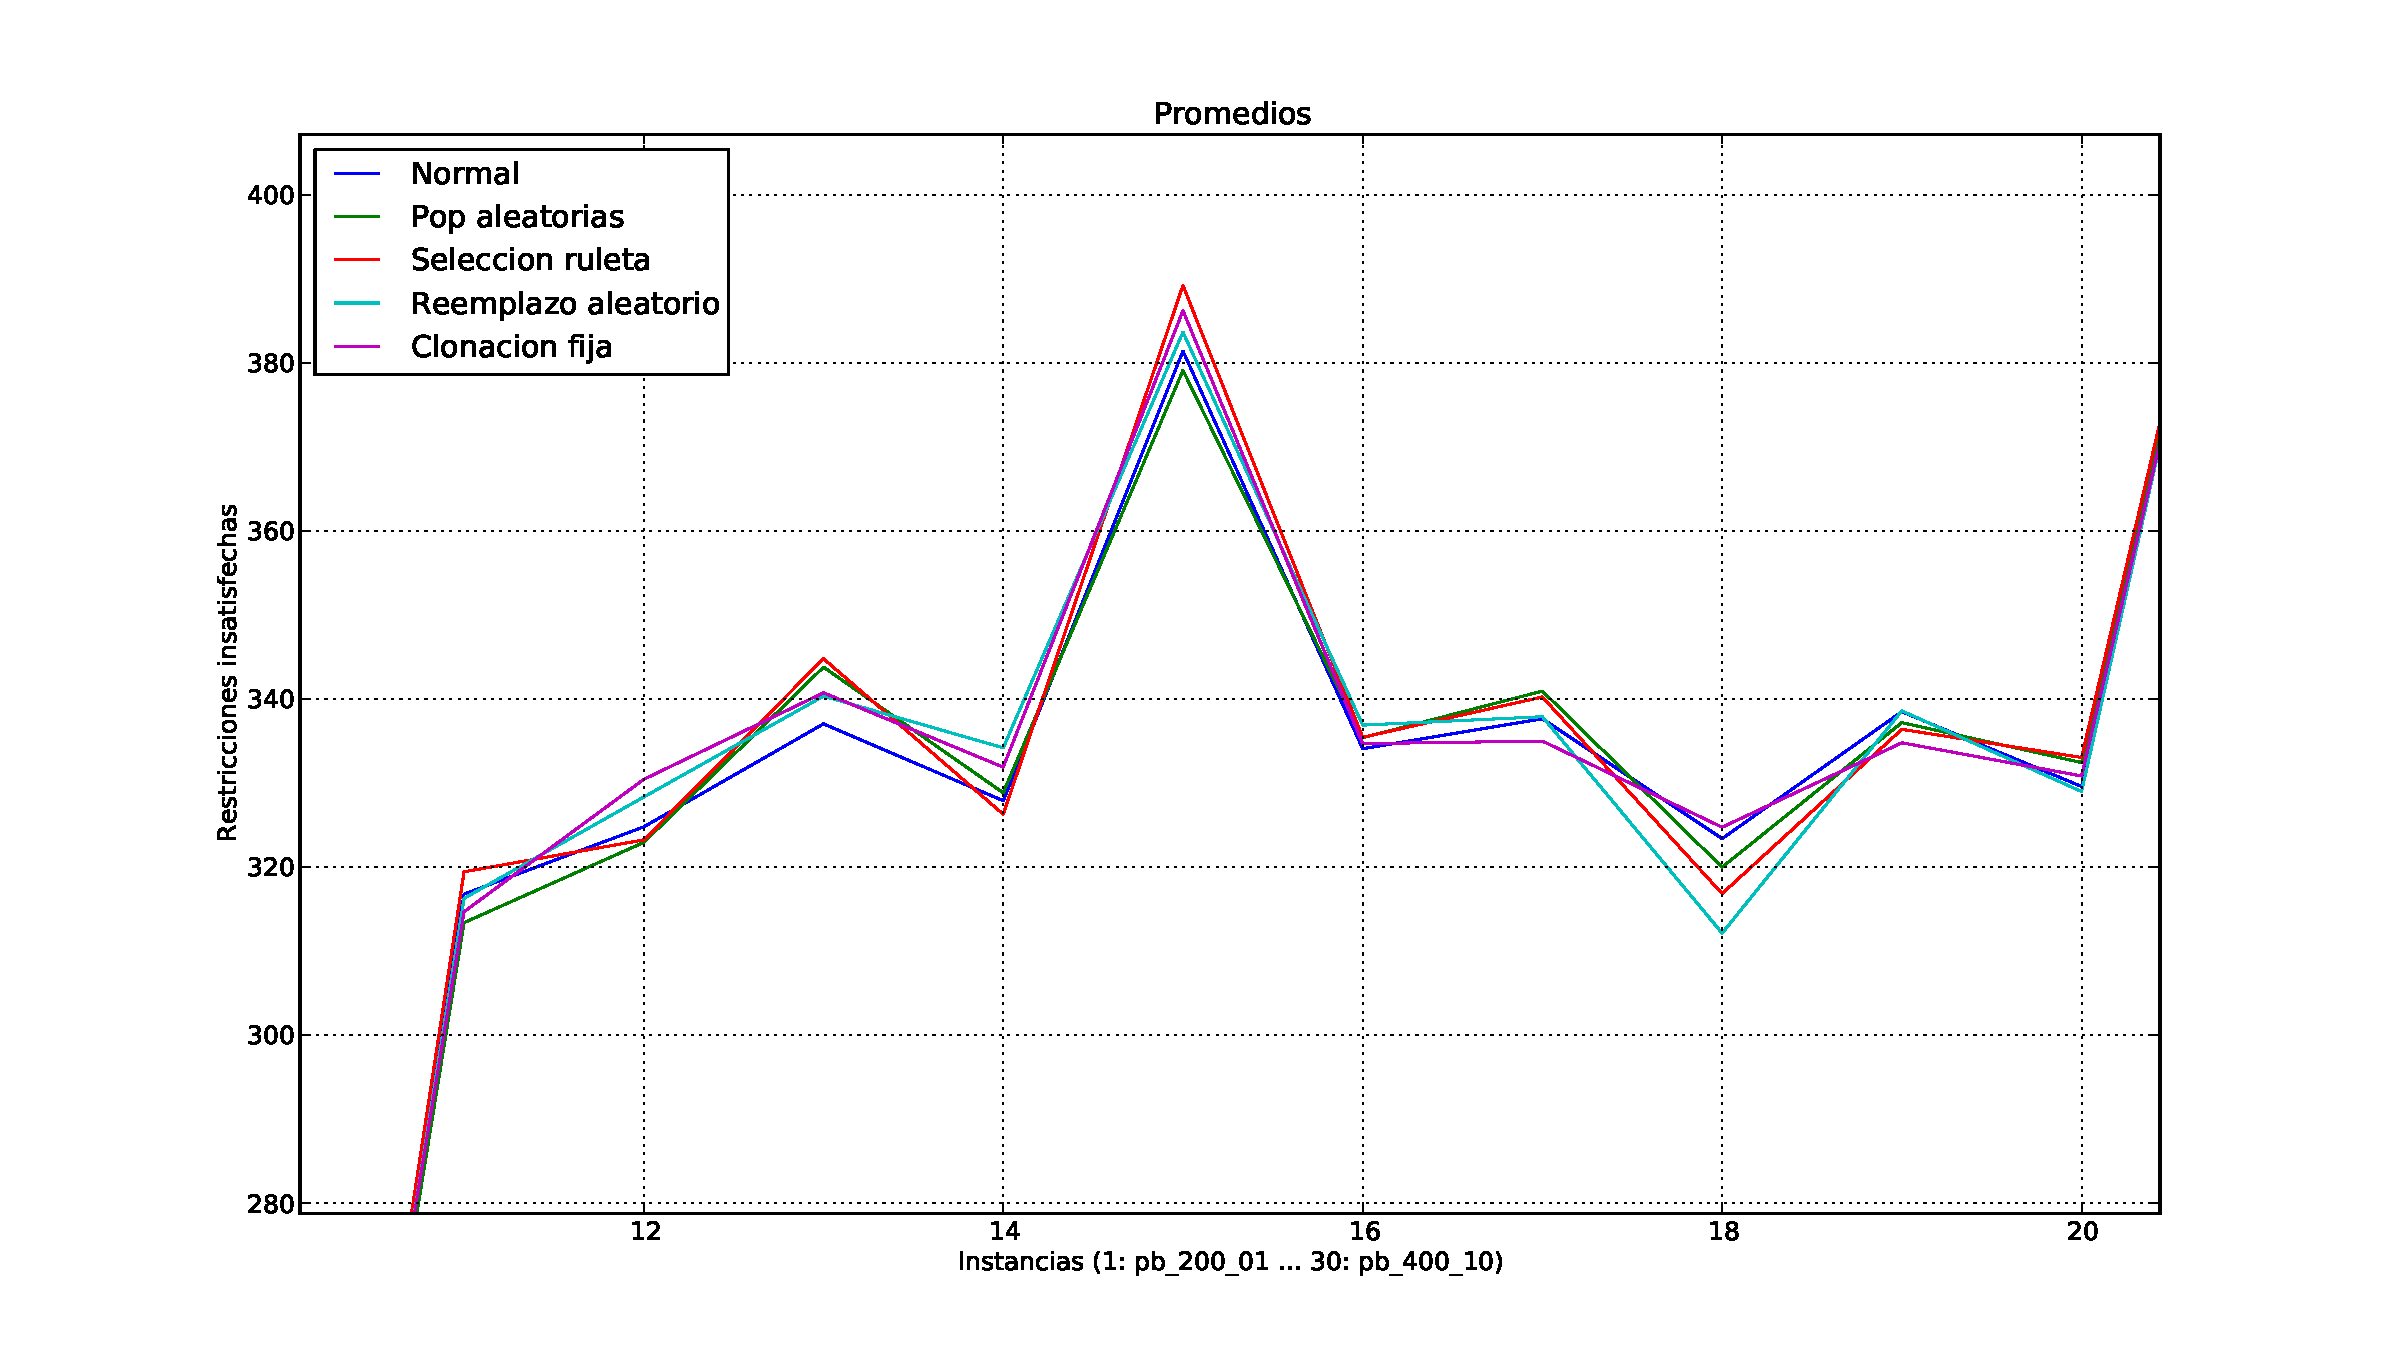
\includegraphics[width=0.95\textwidth]{img/promedio-zoom300.pdf}
\end{center}
\caption{Promedio de valores para cada modificación (Zoom a las instancias de 300)}
\label{fig:promedio300}
\end{figure}

\begin{figure}[H]
\begin{center}
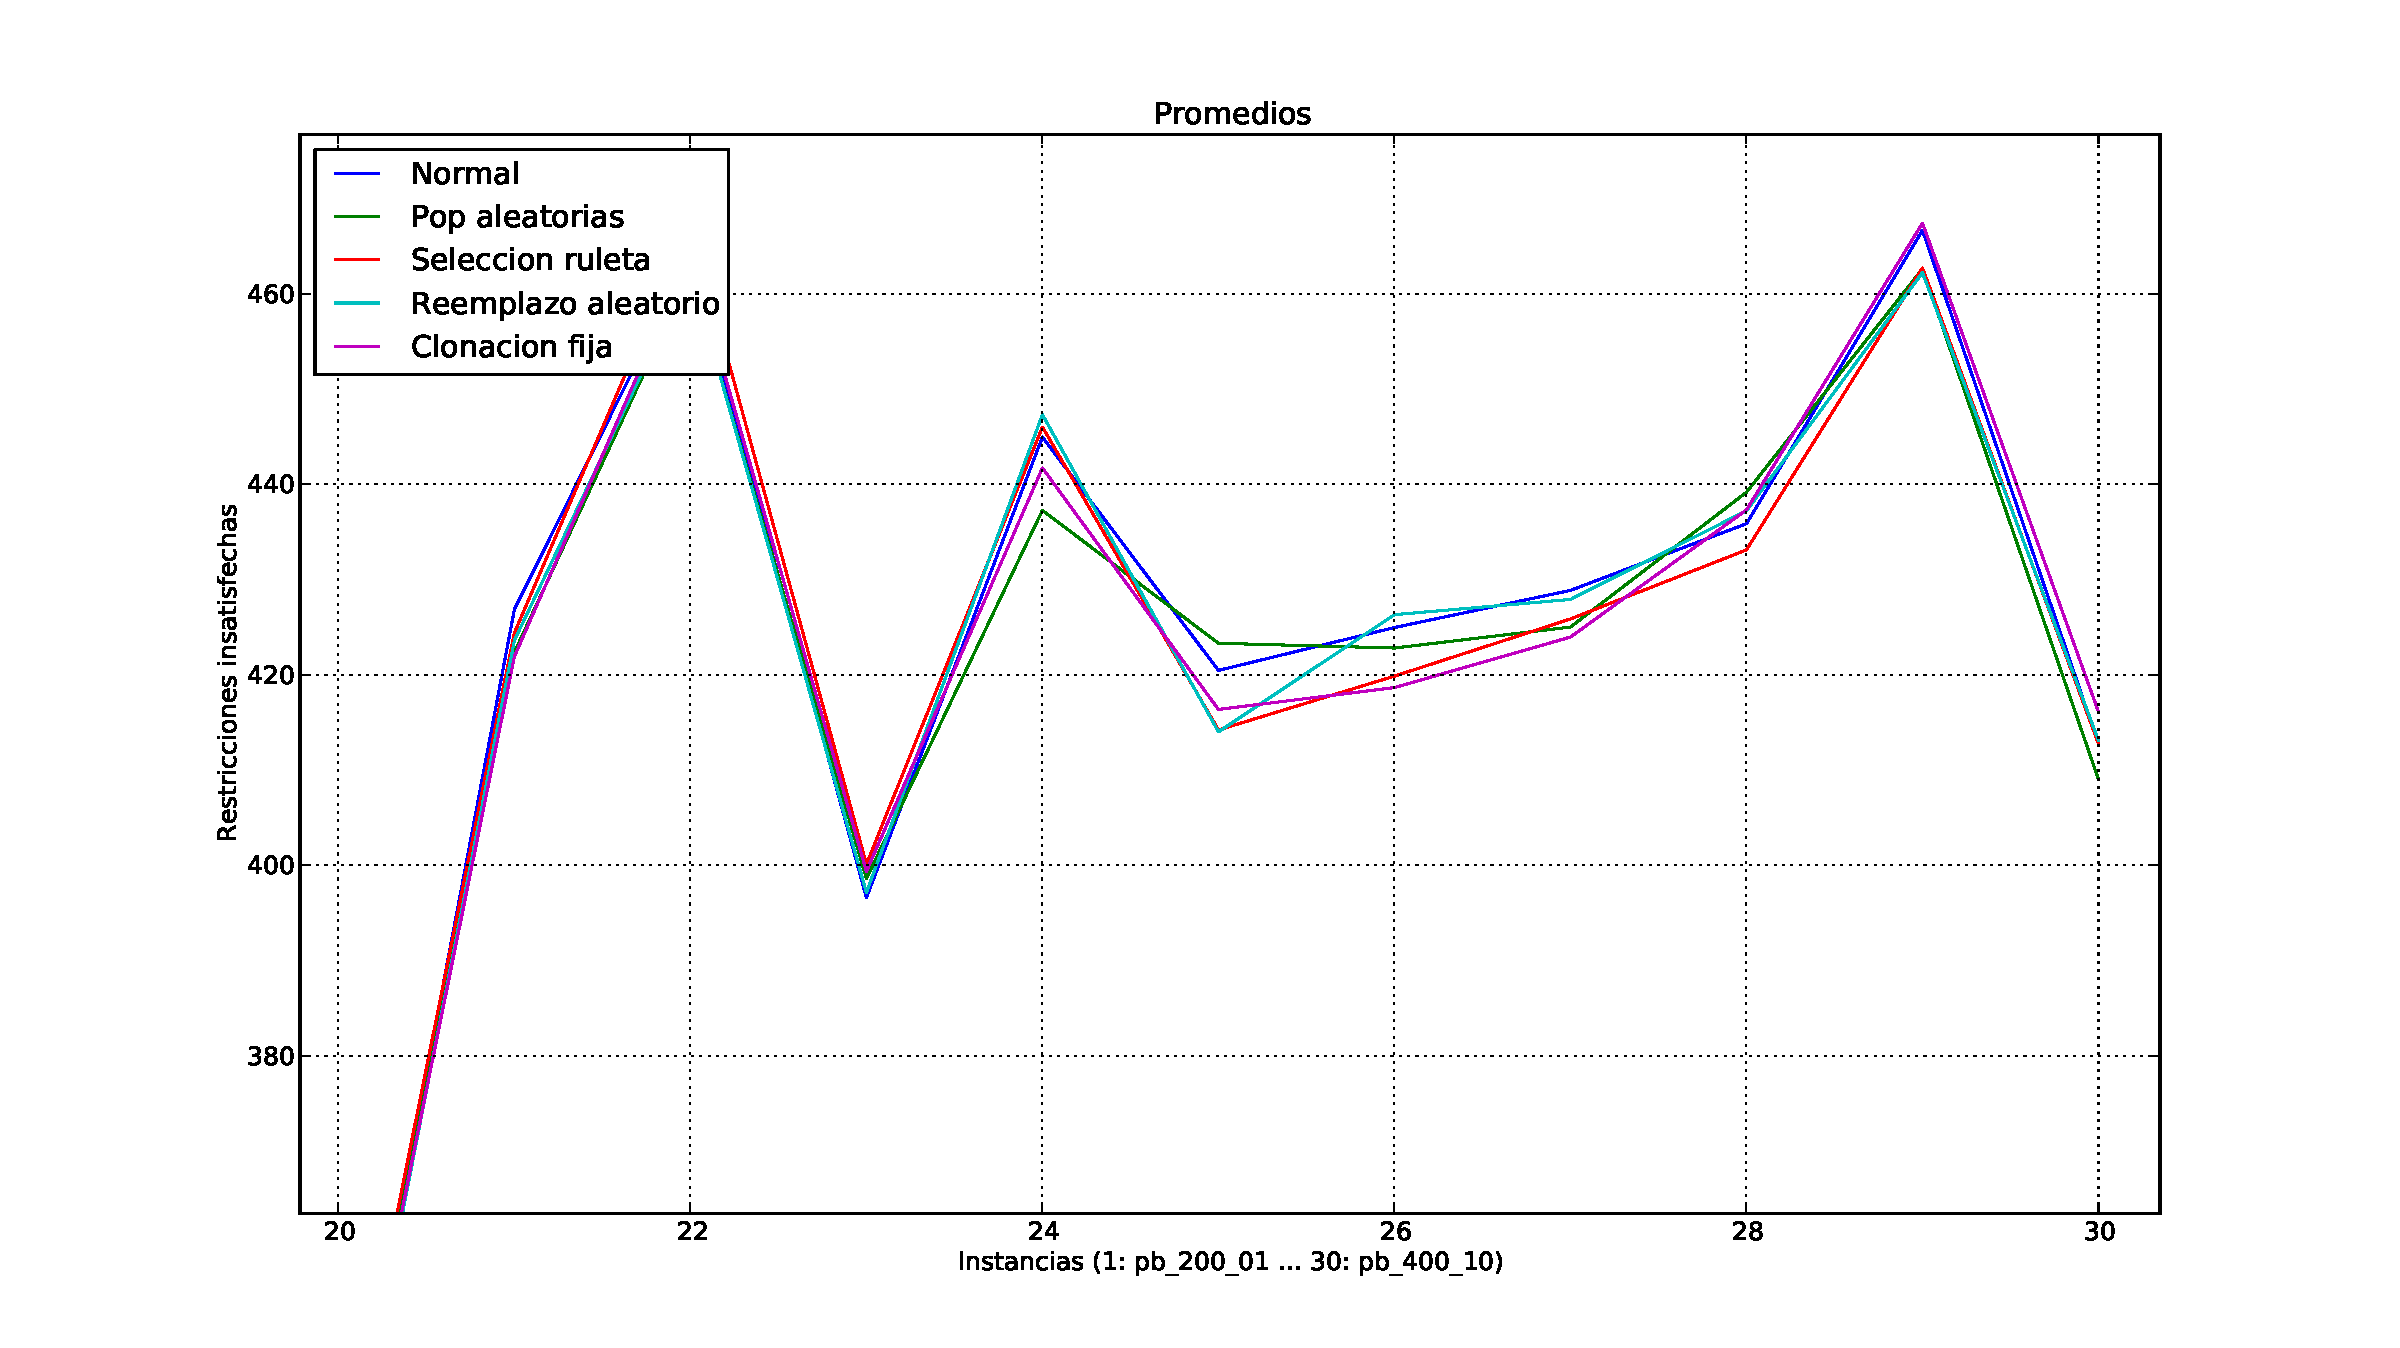
\includegraphics[width=0.95\textwidth]{img/promedio-zoom400.pdf}
\end{center}
\caption{Promedio de valores para cada modificación (Zoom a las instancias de 400)}
\label{fig:promedio400}
\end{figure}

\newpage

\subsection{Desviación estándar}

\begin{figure}[H]
\begin{center}
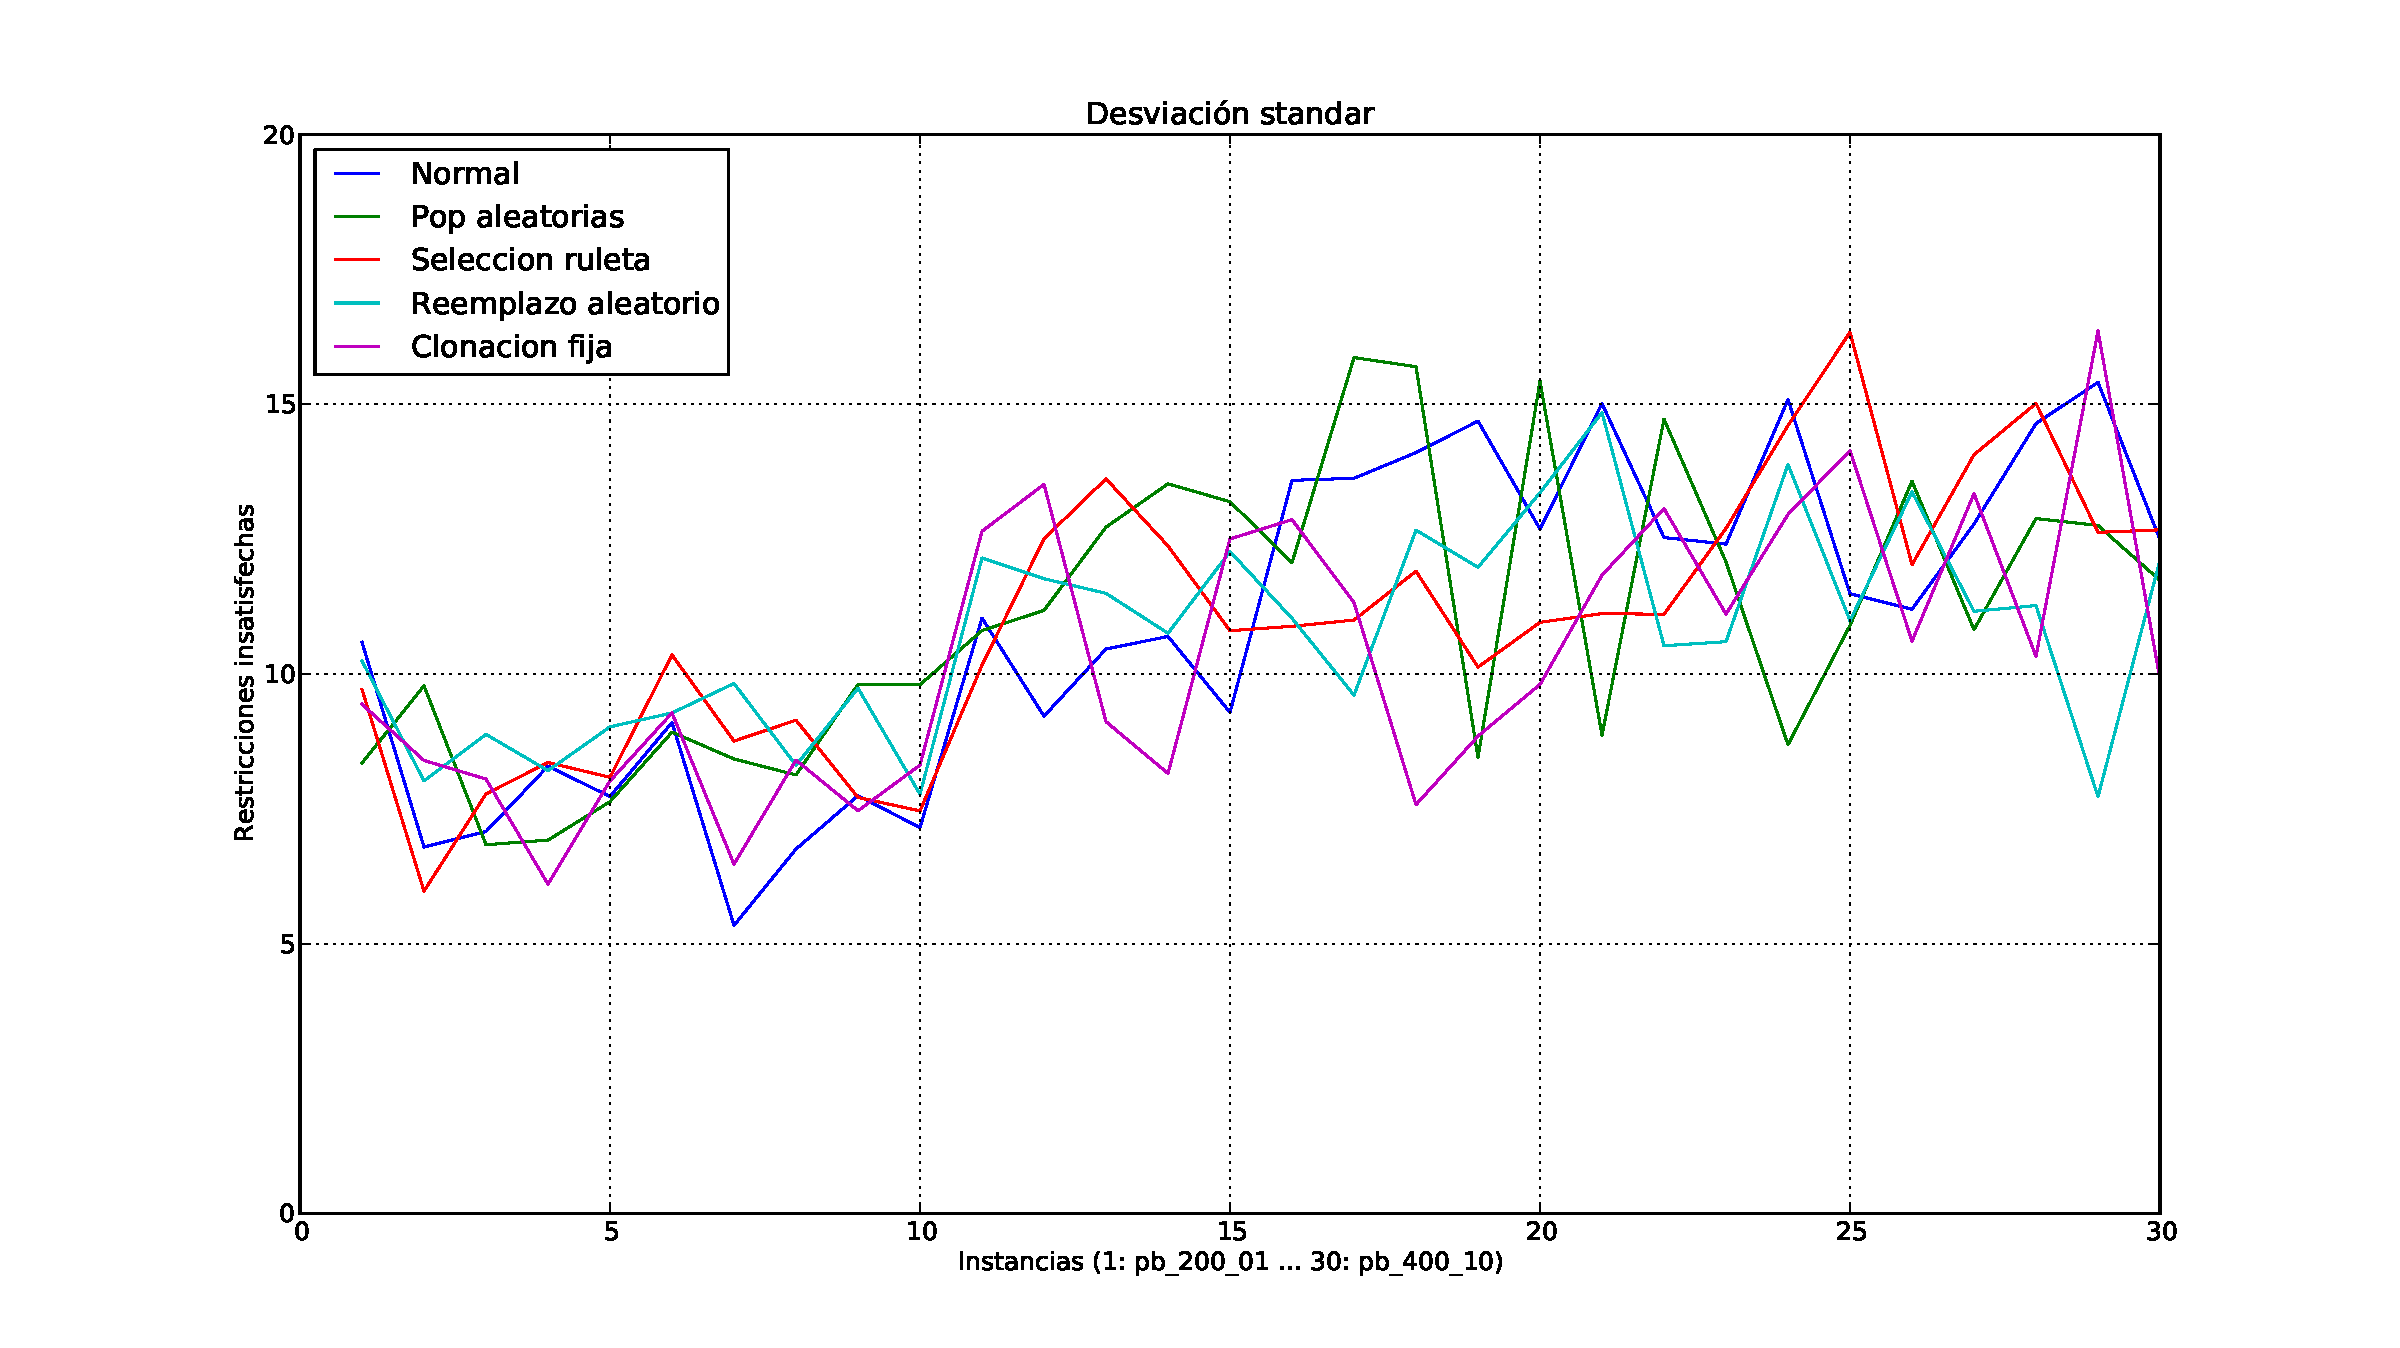
\includegraphics[width=0.95\textwidth]{img/s.pdf}
\end{center}
\caption{Desviación estándar para cada modificación.}
\label{fig:s}
\end{figure}

\newpage

\subsection{Valores máximos}

\begin{figure}[H]
\begin{center}
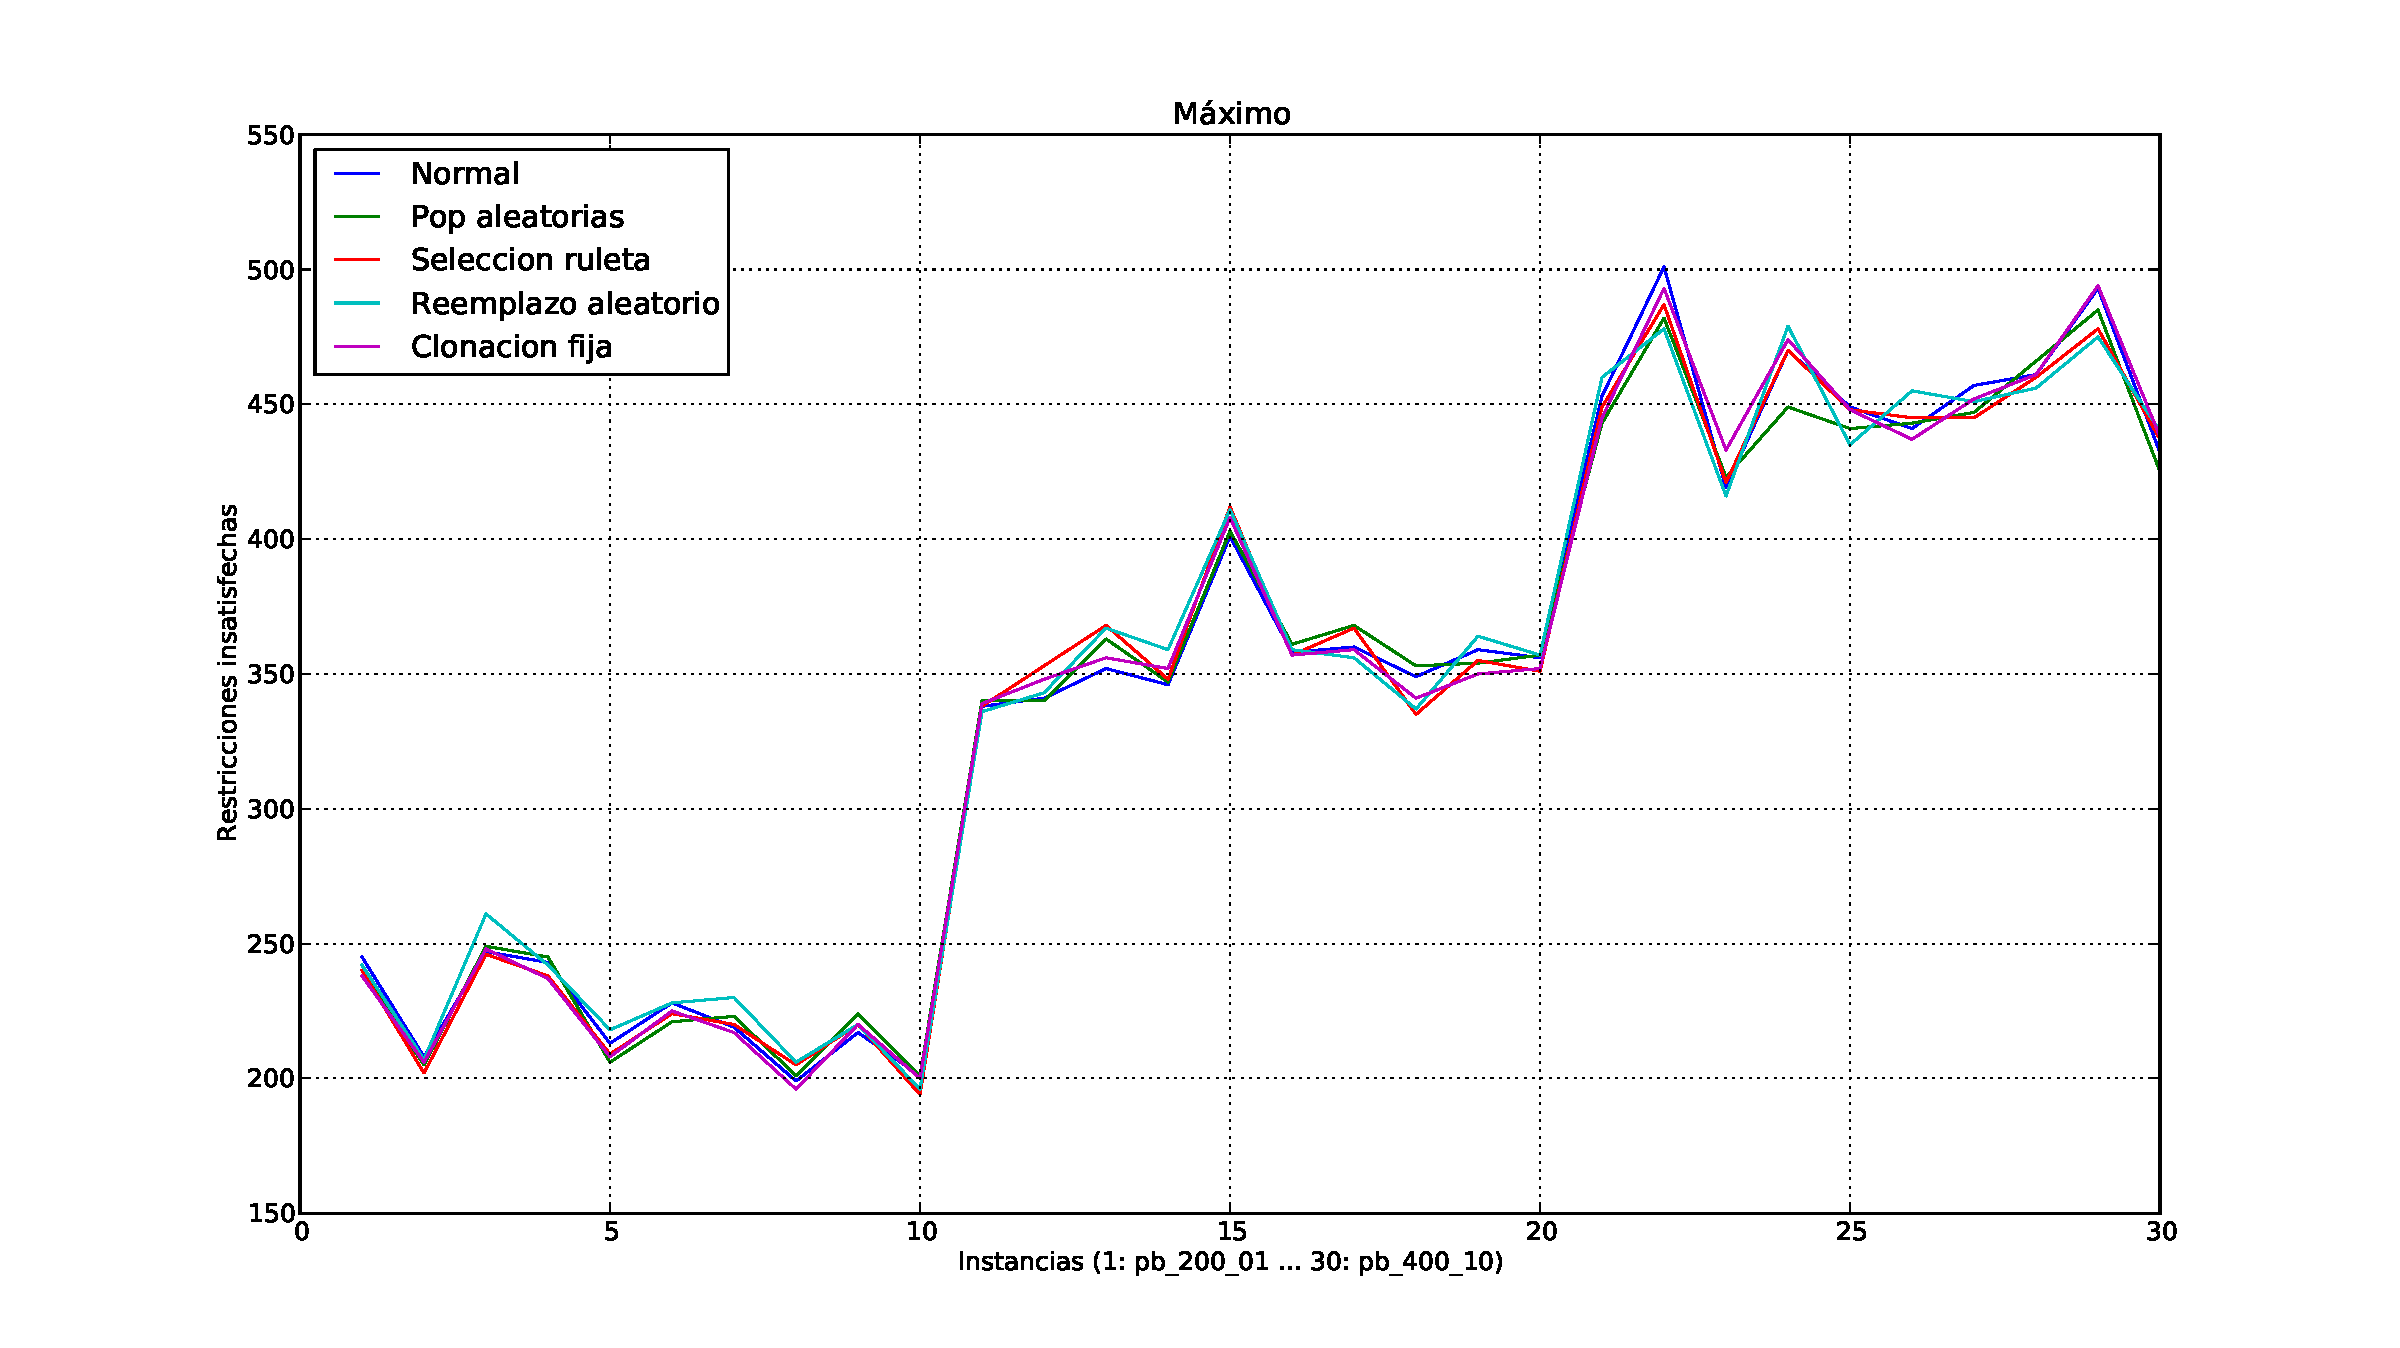
\includegraphics[width=0.95\textwidth]{img/max.pdf}
\end{center}
\caption{Valores máximos para cada modificación}
\label{fig:max}
\end{figure}

\begin{figure}[H]
\begin{center}
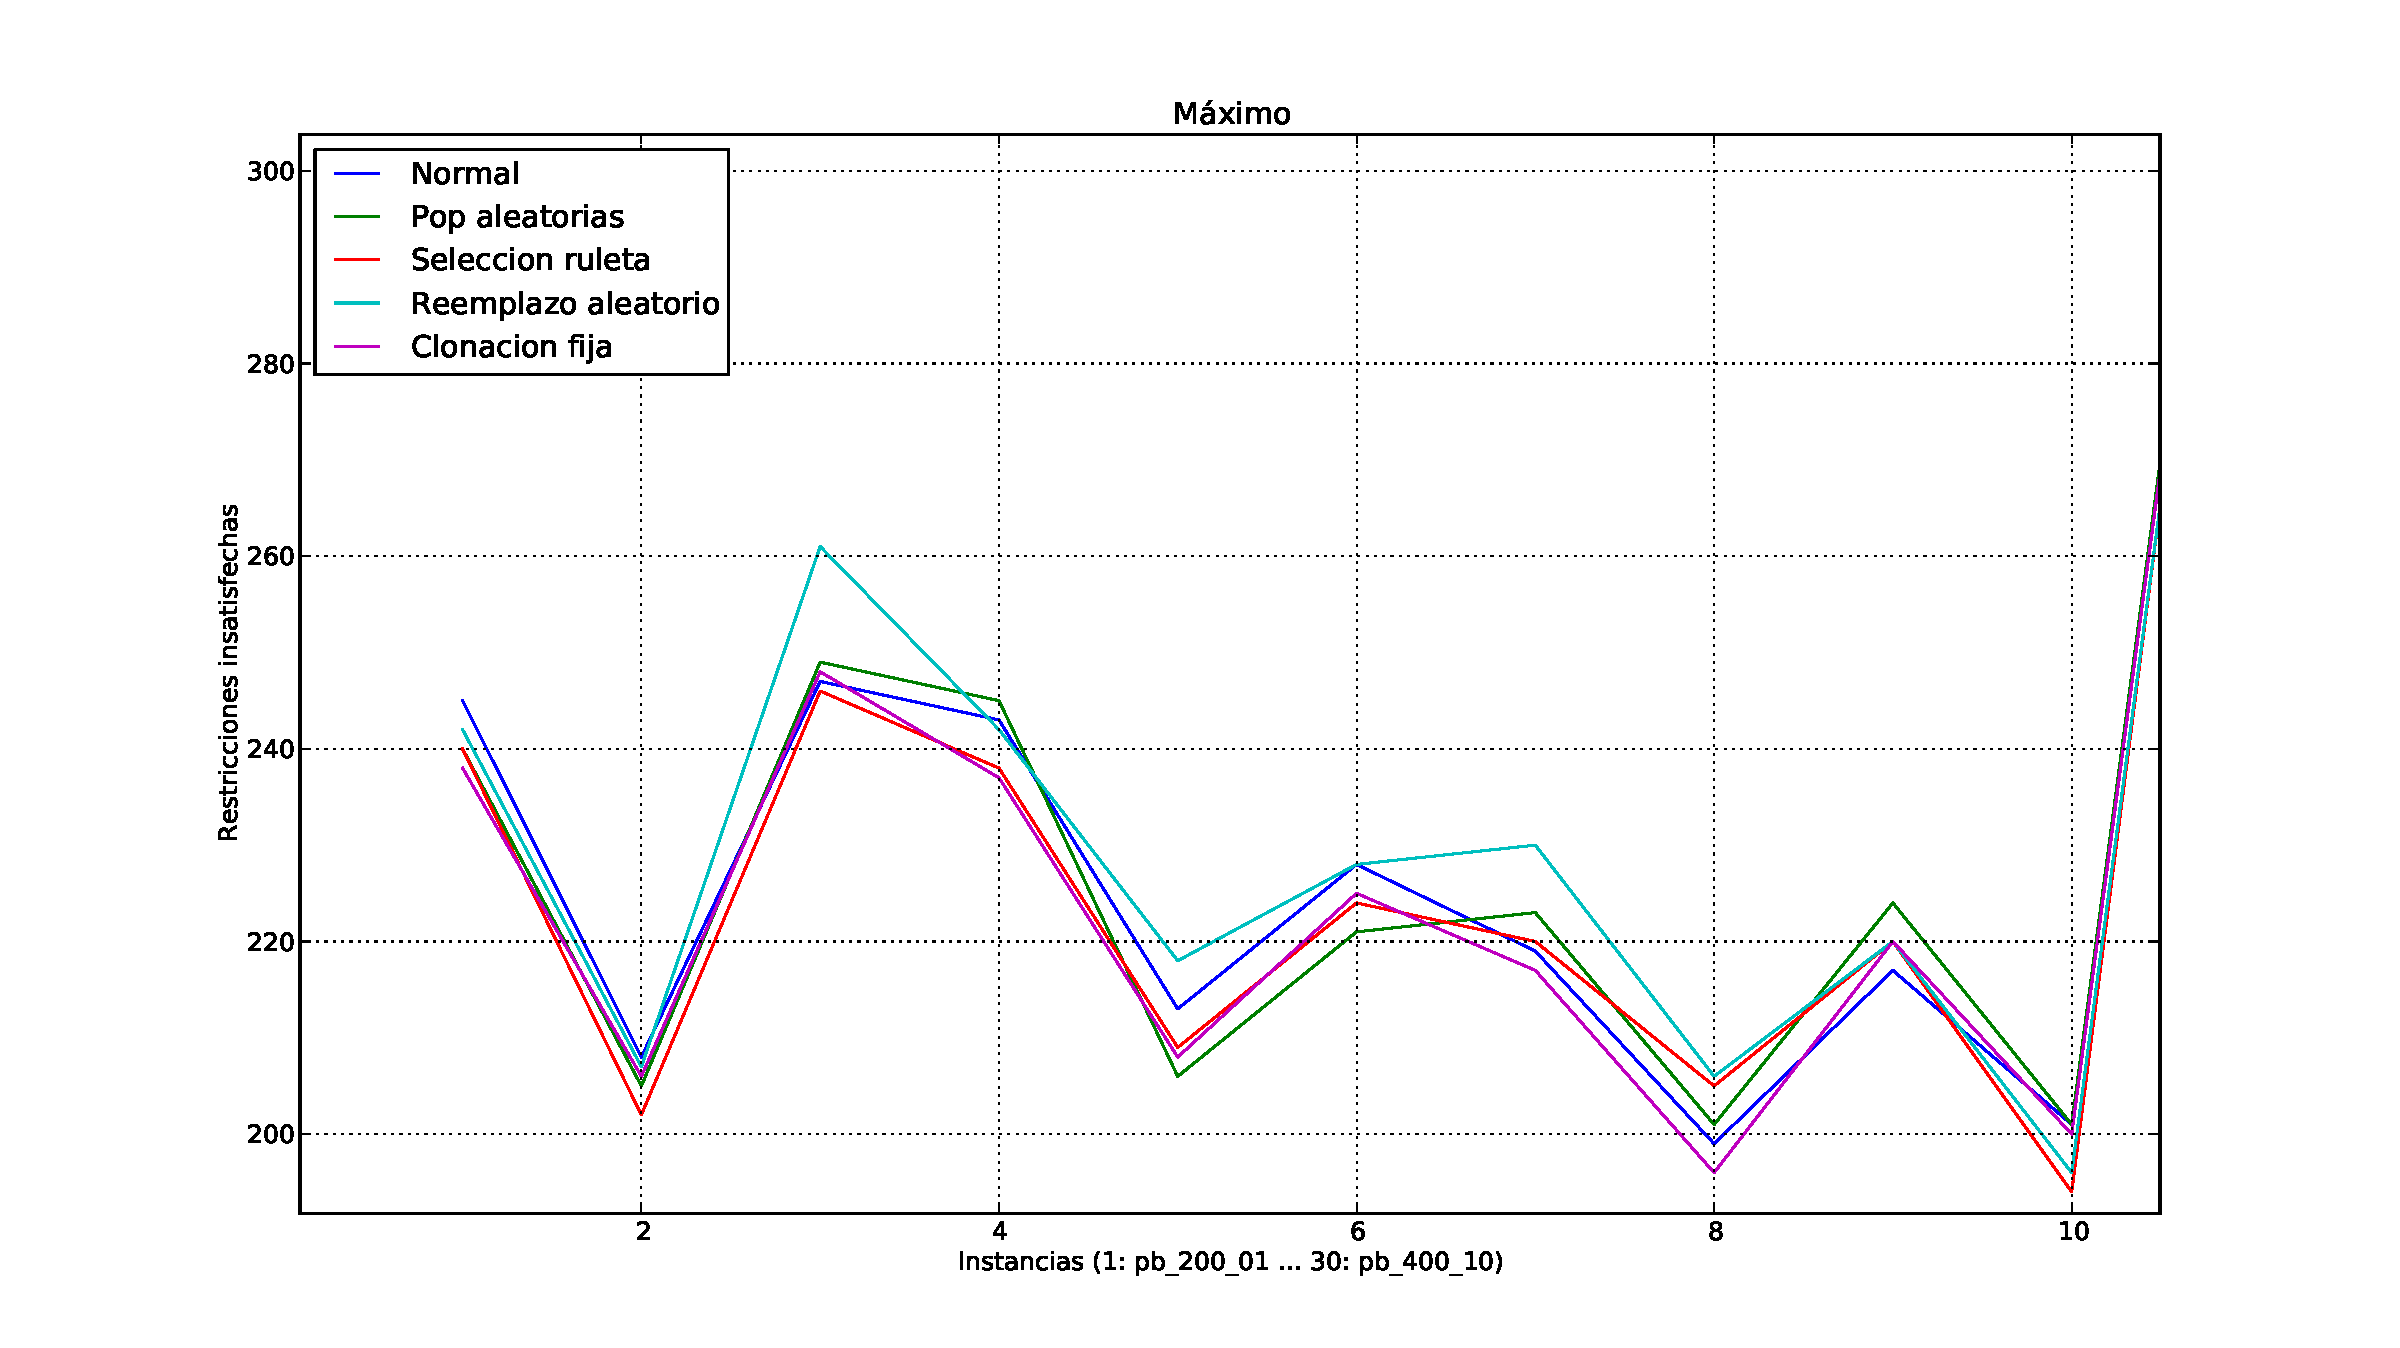
\includegraphics[width=0.95\textwidth]{img/max-zoom200.pdf}
\end{center}
\caption{Valores máximos para cada modificación (Zoom a las instancias de 200)}
\label{fig:max200}
\end{figure}

\begin{figure}[H]
\begin{center}
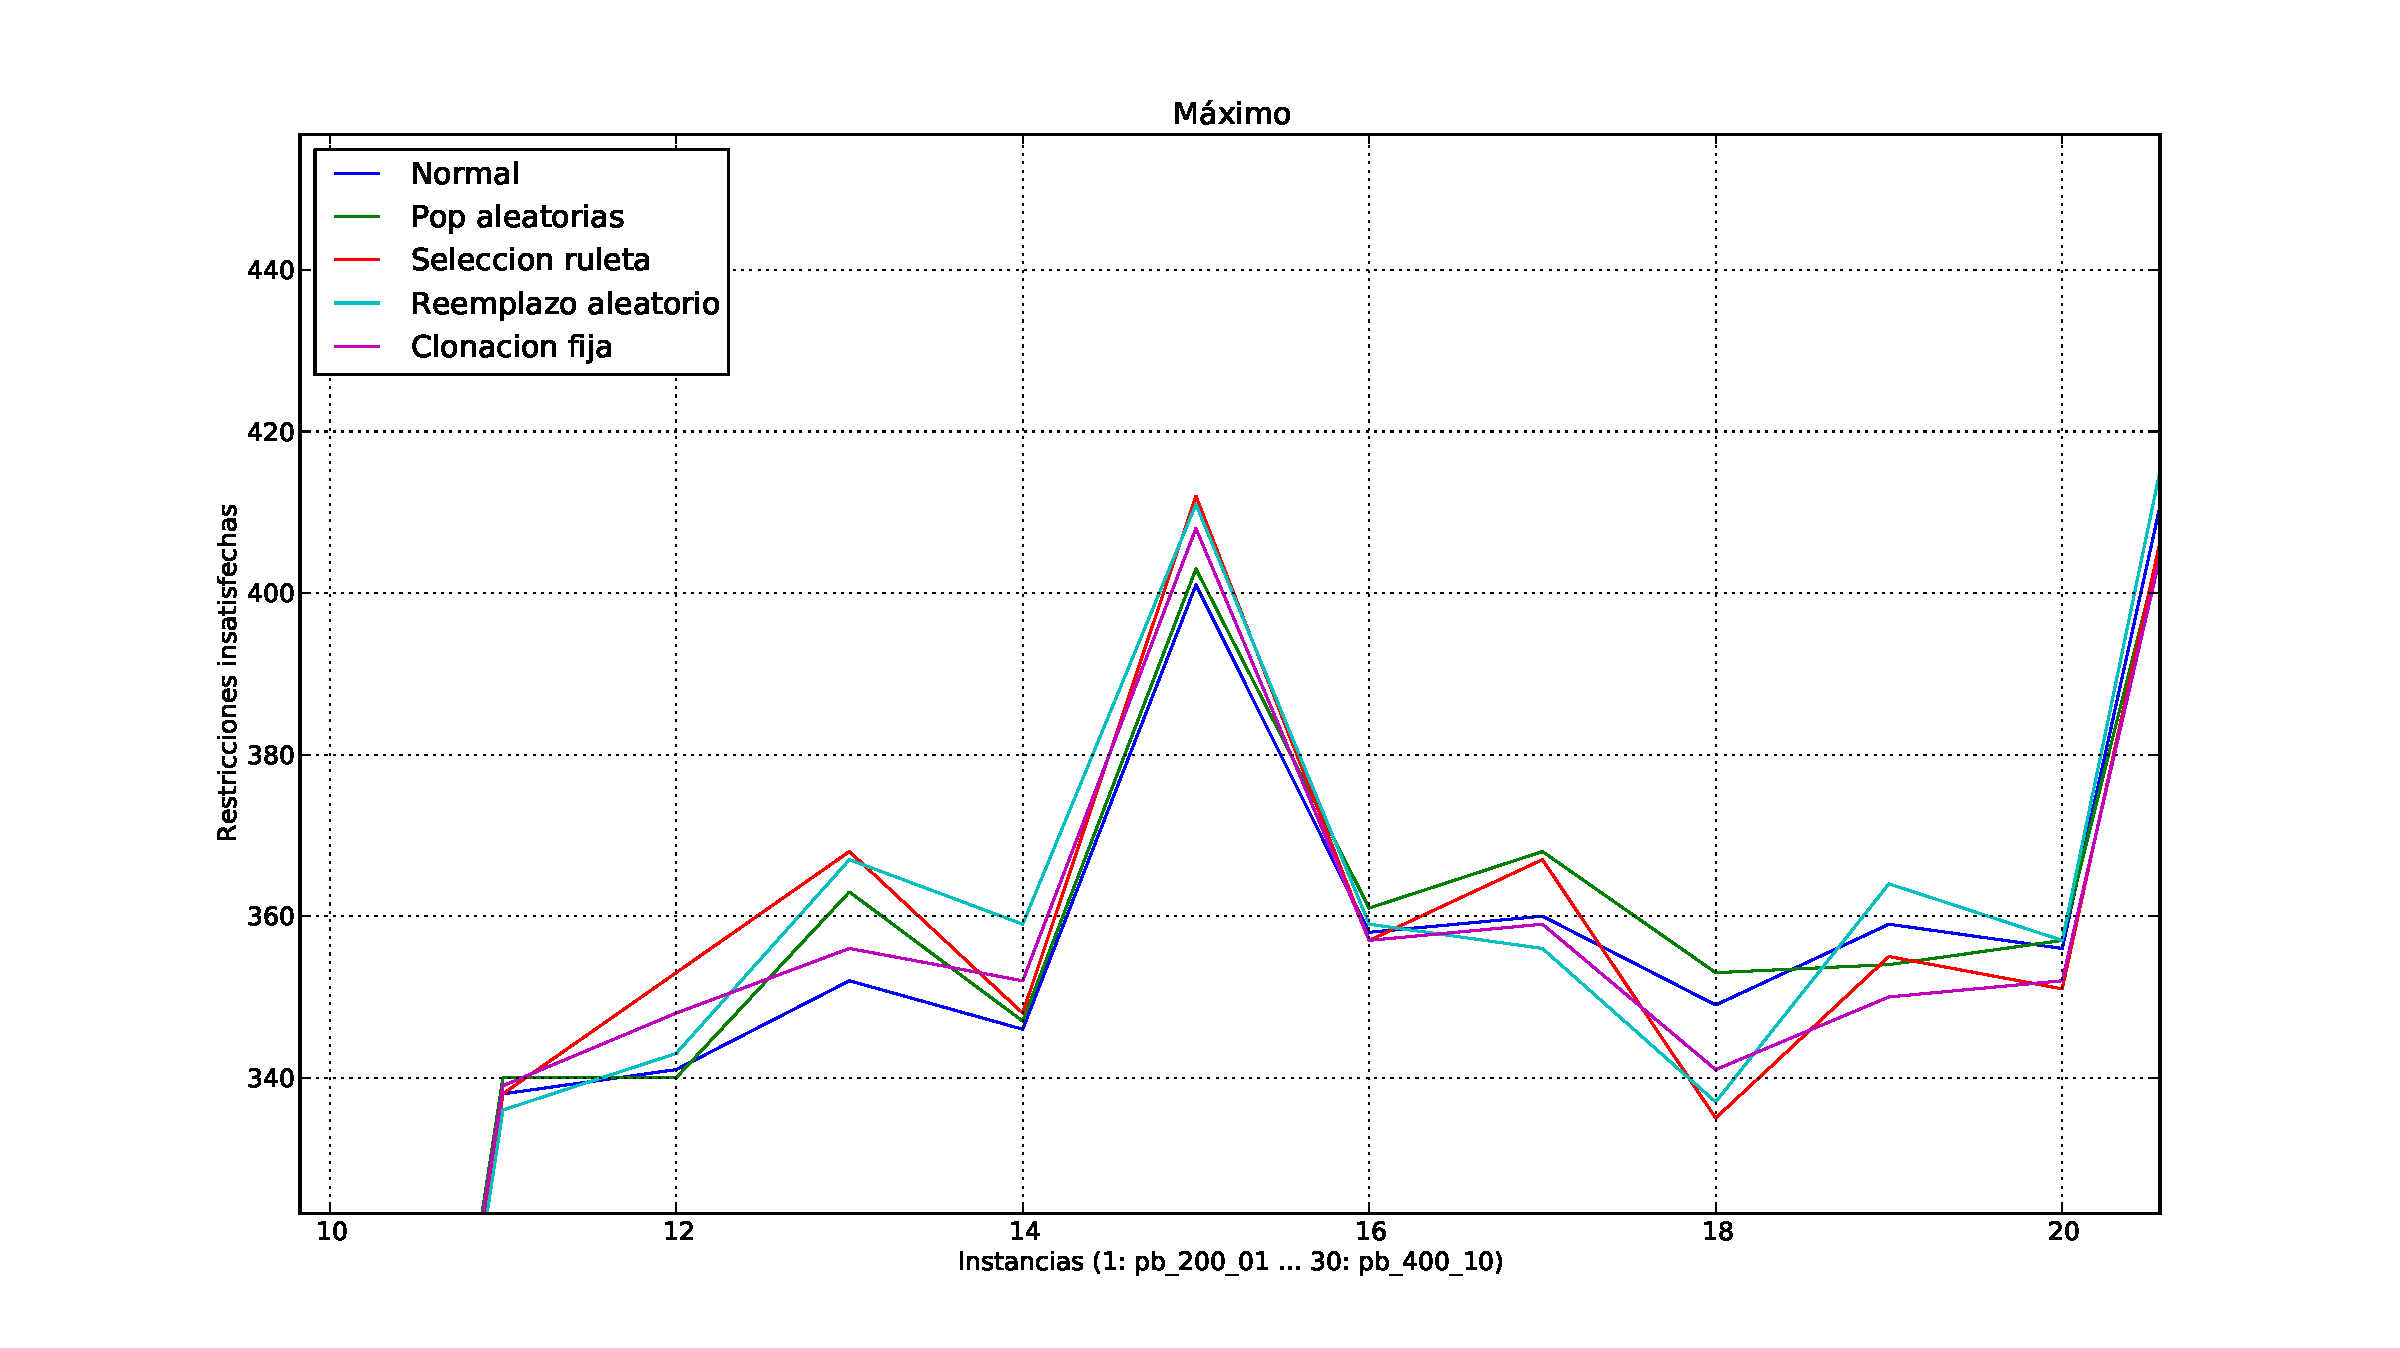
\includegraphics[width=0.95\textwidth]{img/max-zoom300.pdf}
\end{center}
\caption{Valores máximos para cada modificación (Zoom a las instancias de 300)}
\label{fig:max300}
\end{figure}

\begin{figure}[H]
\begin{center}
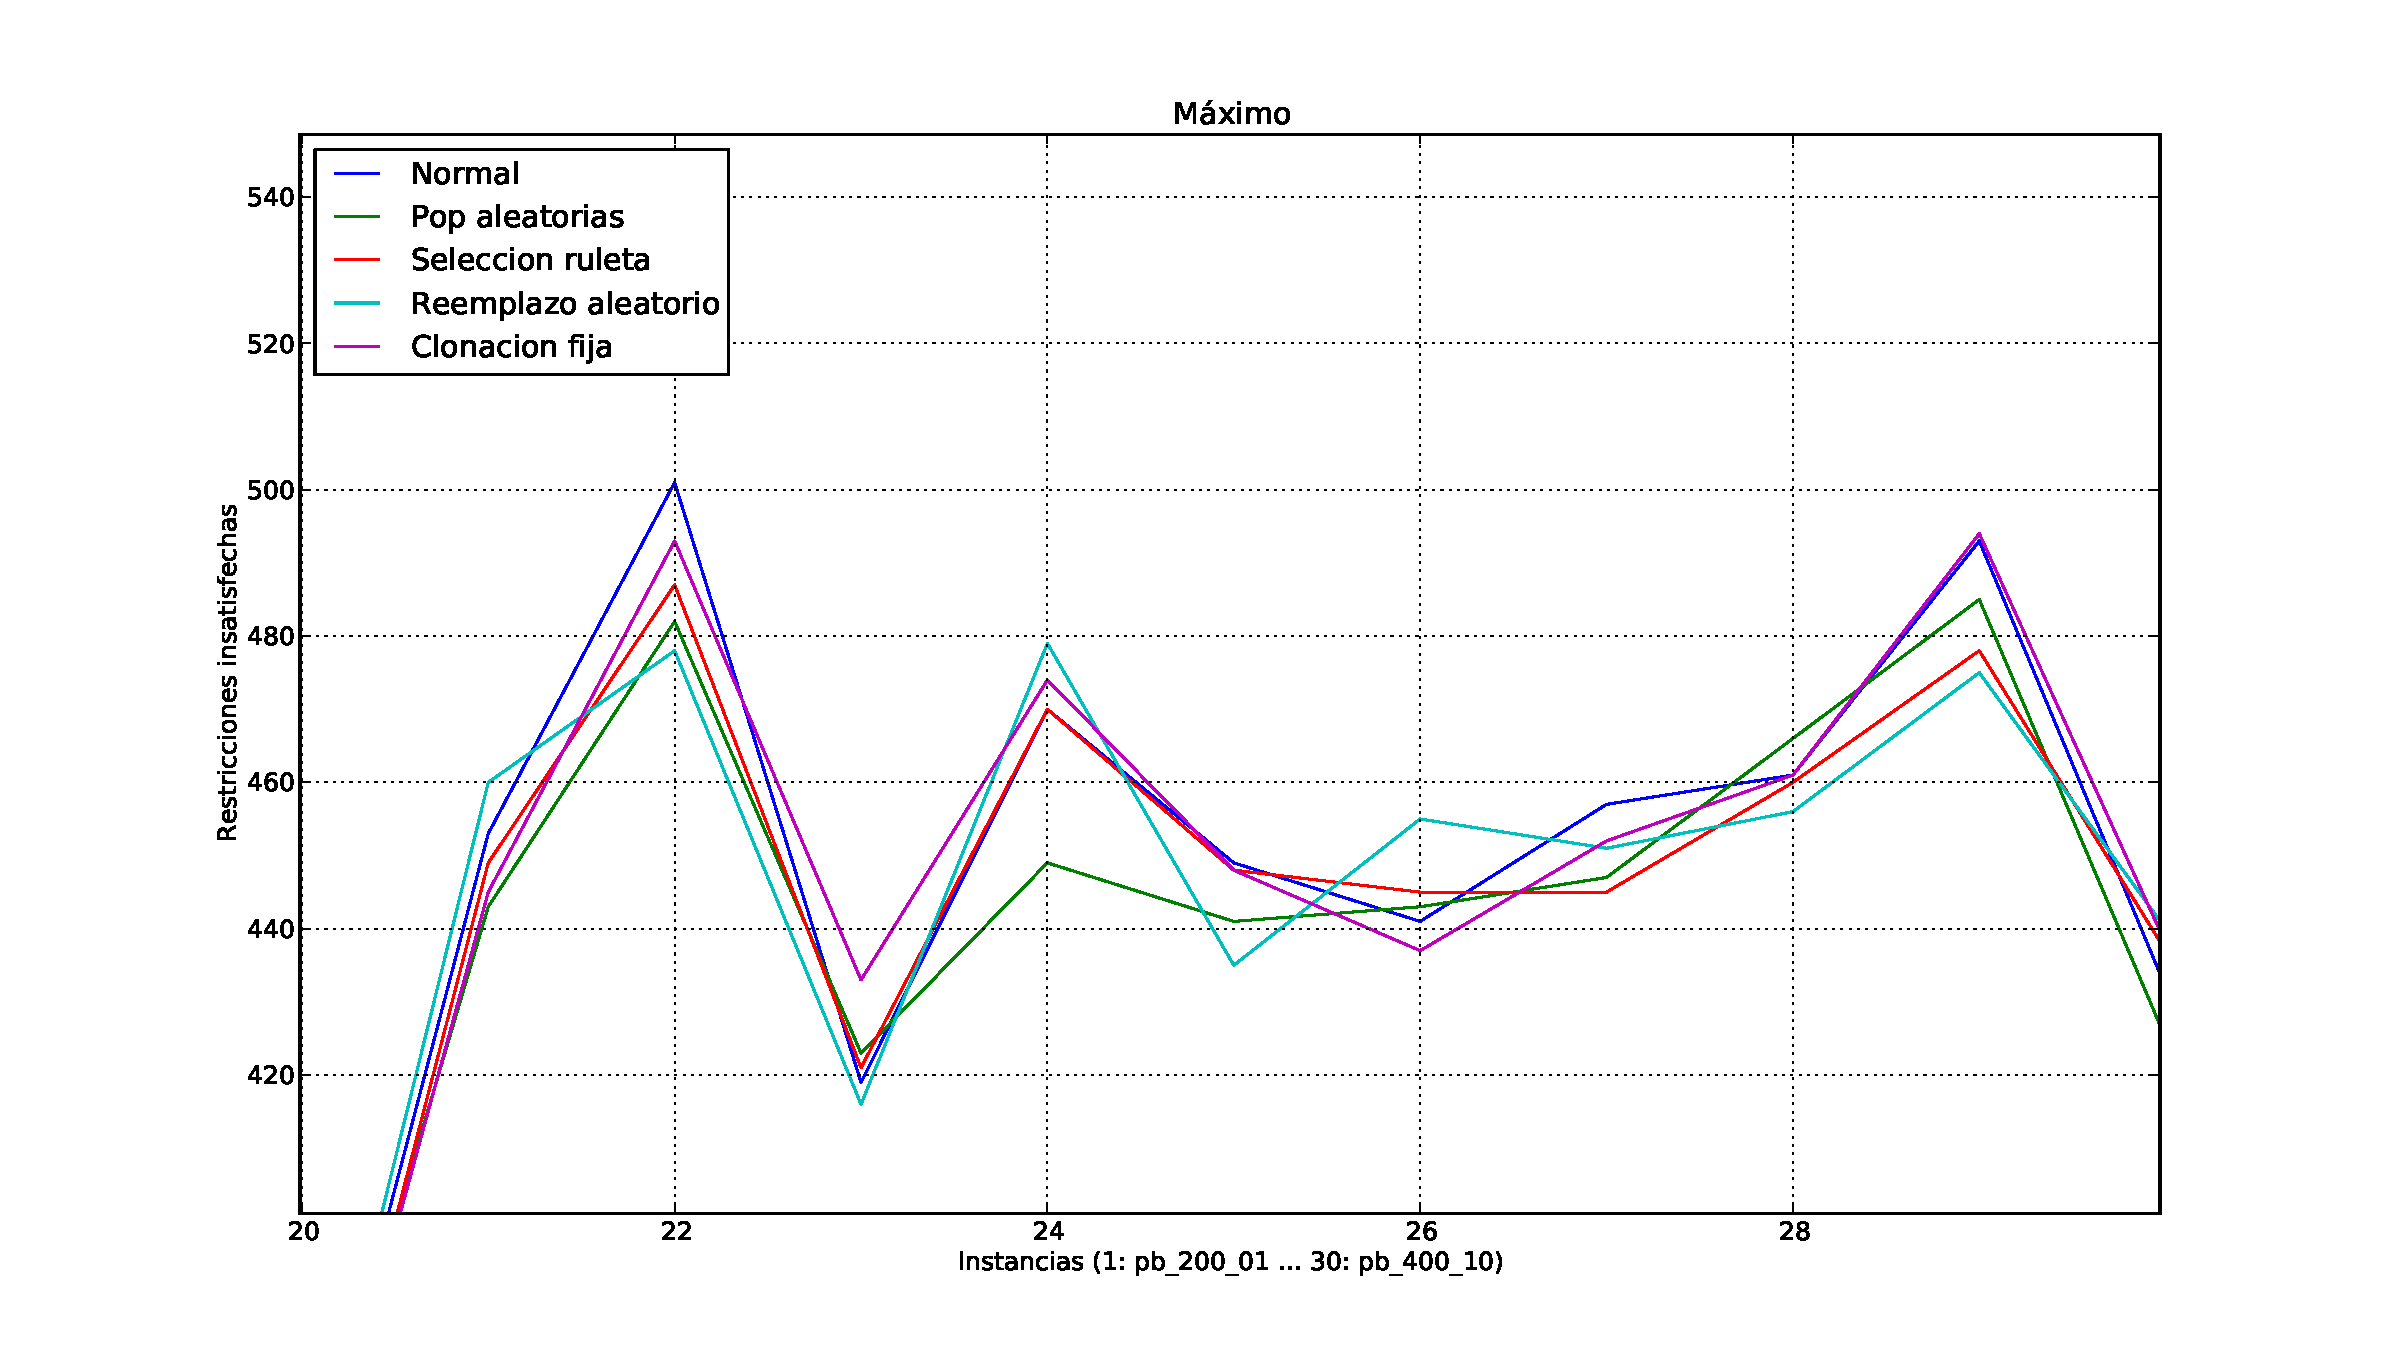
\includegraphics[width=0.95\textwidth]{img/max-zoom400.pdf}
\end{center}
\caption{Valores máximos para cada modificación (Zoom a las instancias de 400)}
\label{fig:max400}
\end{figure}

\newpage

\subsection{Valores mínimos}

\begin{figure}[H]
\begin{center}
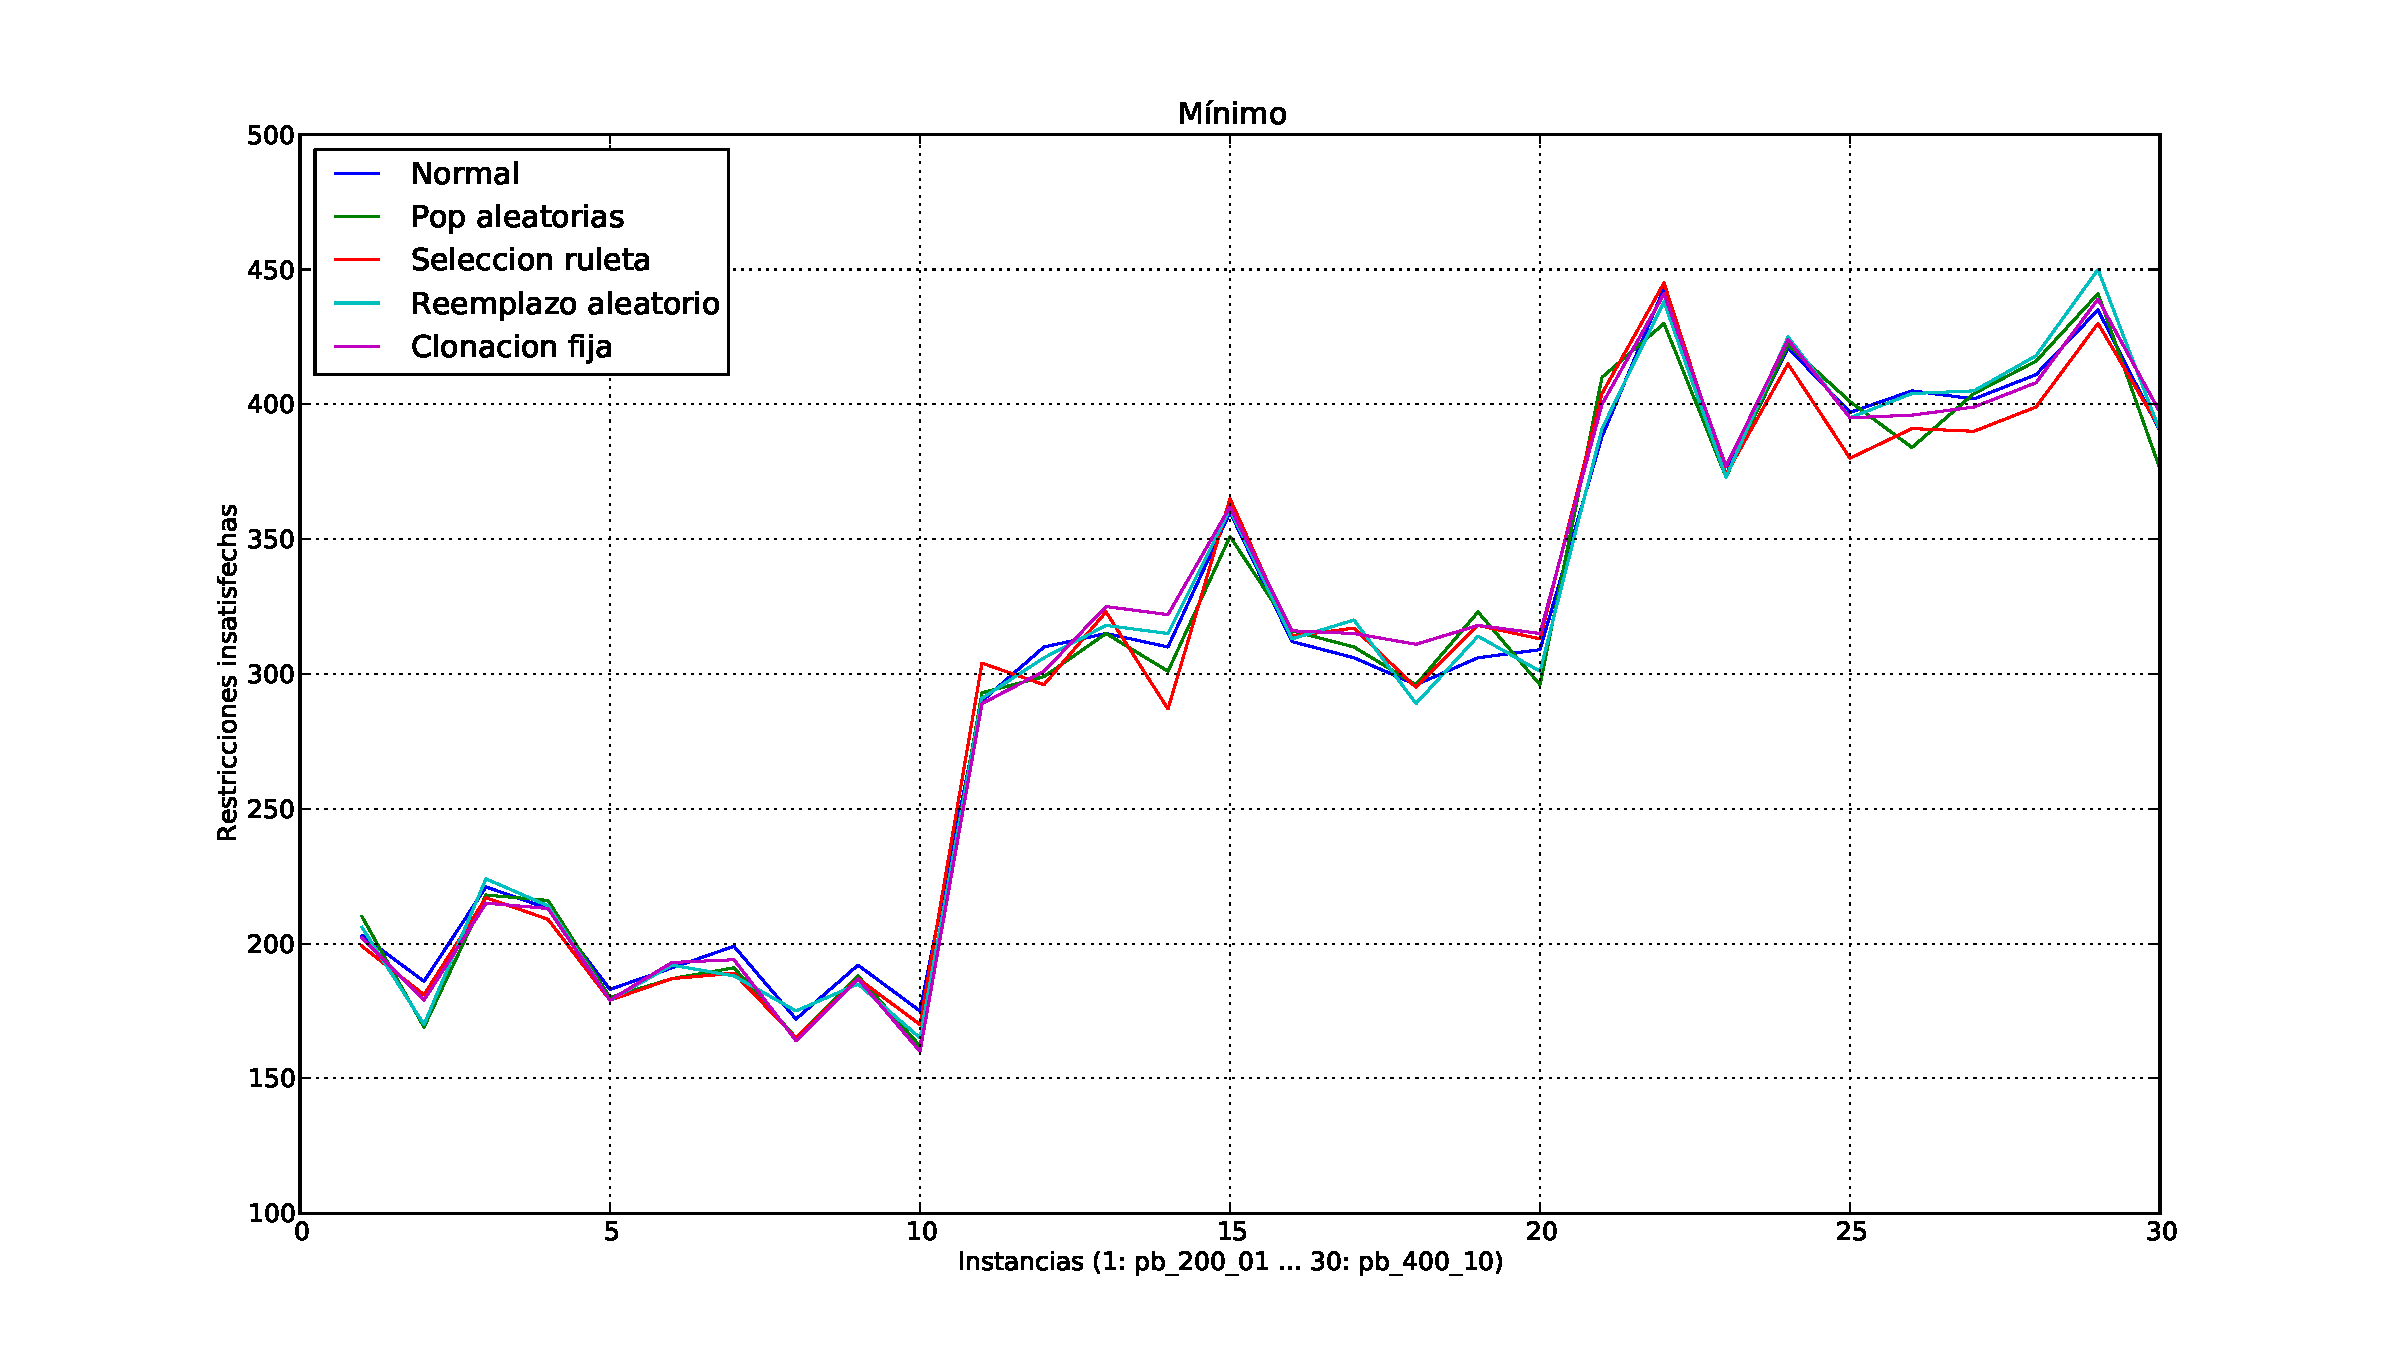
\includegraphics[width=0.8\textwidth]{img/min.pdf}
\end{center}
\caption{Valores mínimos para cada modificación}
\label{fig:min}
\end{figure}

\begin{figure}[H]
\begin{center}
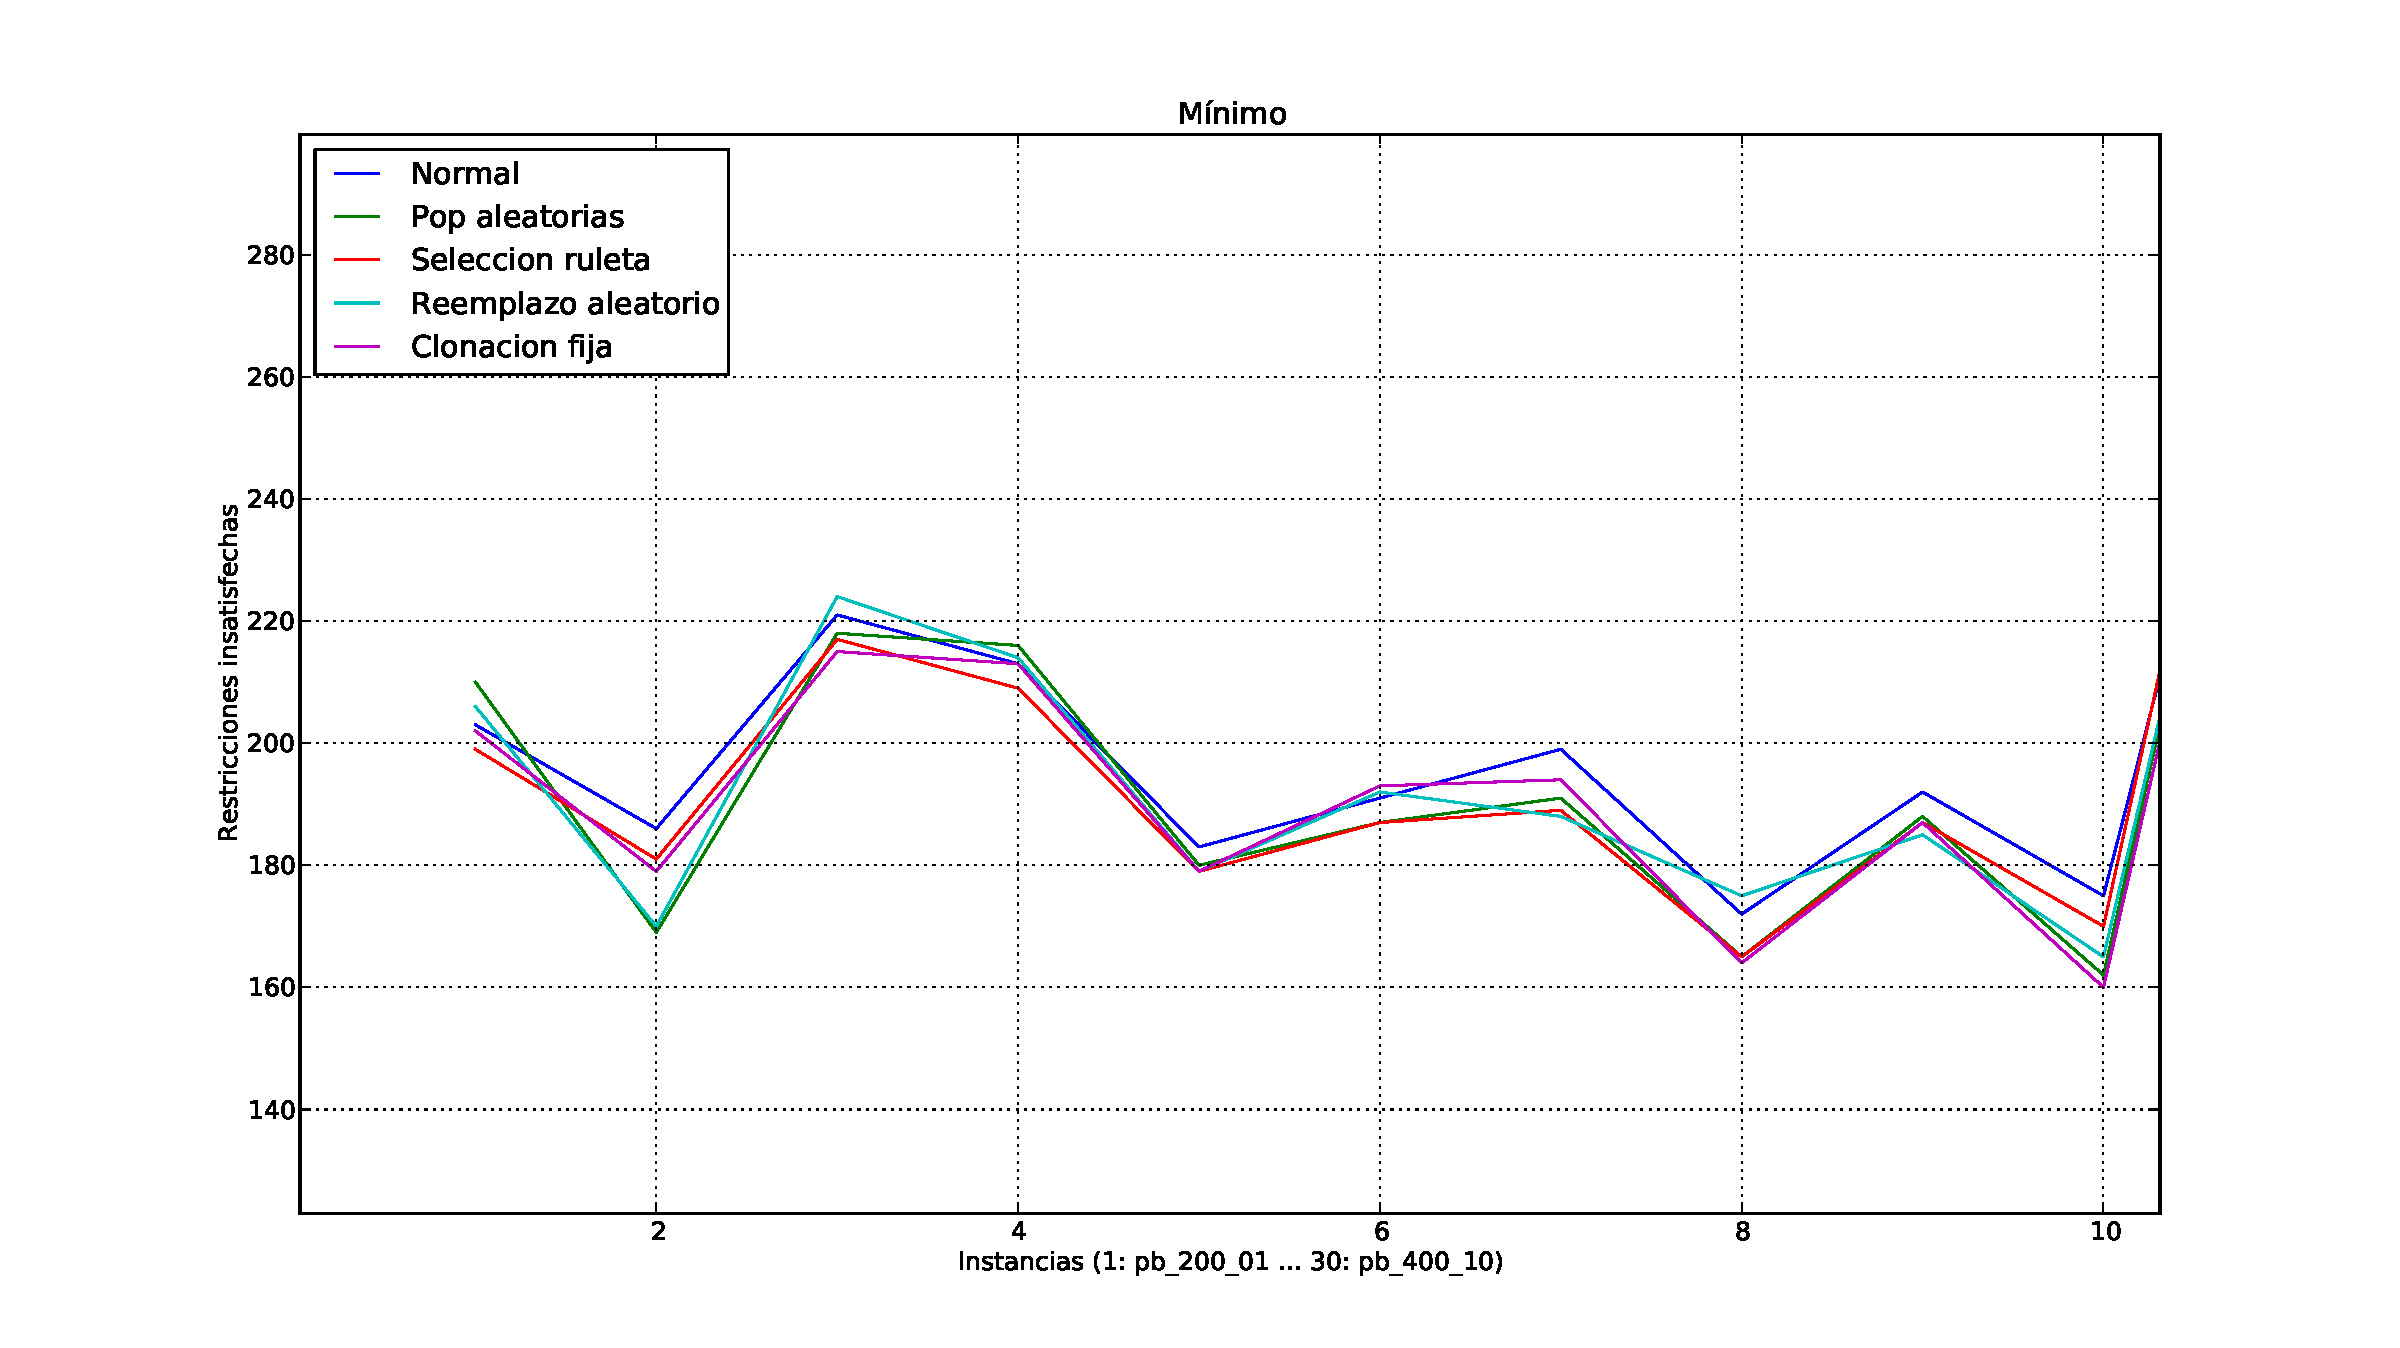
\includegraphics[width=0.8\textwidth]{img/min-zoom200.pdf}
\end{center}
\caption{Valores mínimos para cada modificación (Zoom a las instancias de 200)}
\label{fig:min200}
\end{figure}

\begin{figure}[H]
\begin{center}
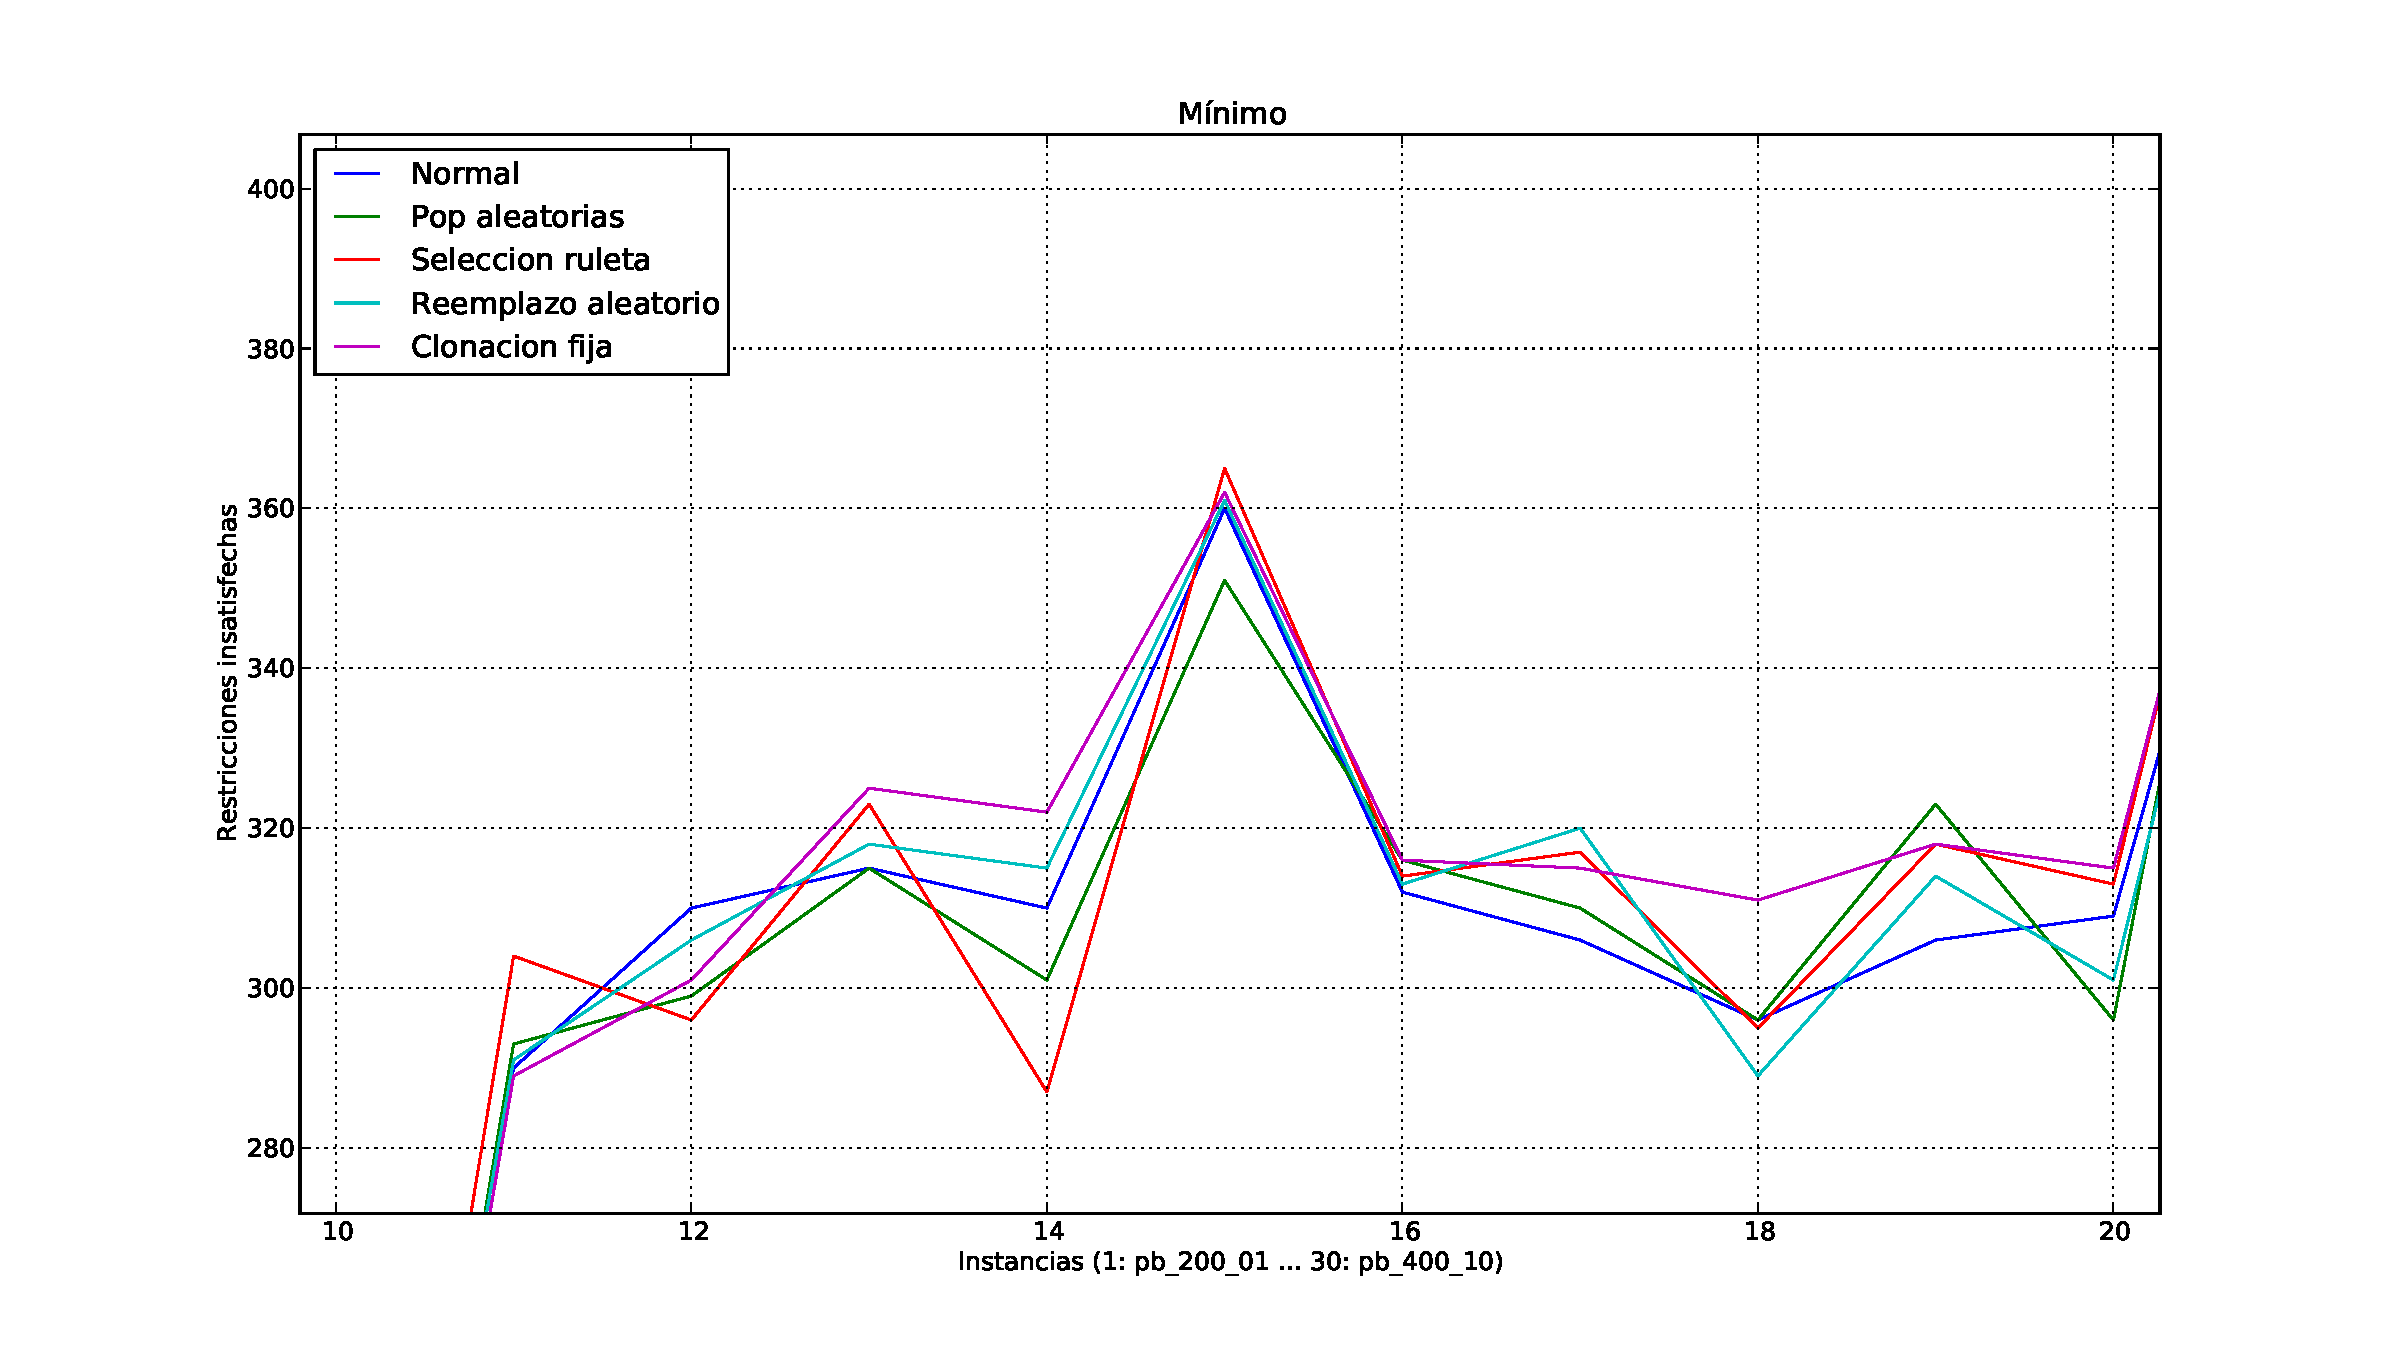
\includegraphics[width=0.8\textwidth]{img/min-zoom300.pdf}
\end{center}
\caption{Valores mínimos para cada modificación (Zoom a las instancias de 300)}
\label{fig:min300}
\end{figure}

\begin{figure}[H]
\begin{center}
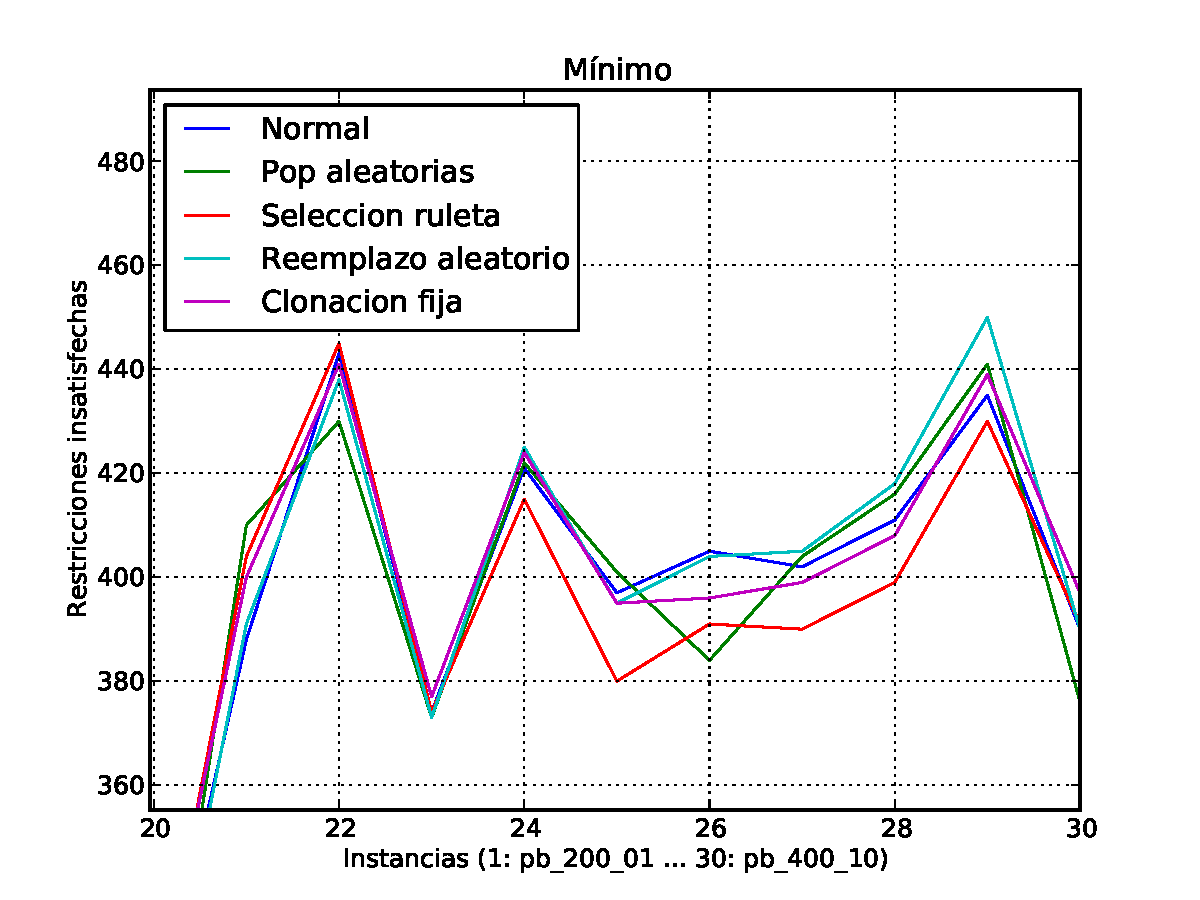
\includegraphics[width=0.8\textwidth]{img/min-zoom400.pdf}
\end{center}
\caption{Valores mínimos para cada modificación (Zoom a las instancias de 400)}
\label{fig:min400}
\end{figure}

\newpage
\subsection{Tiempo de ejecución}

\begin{figure}[H]
\begin{center}
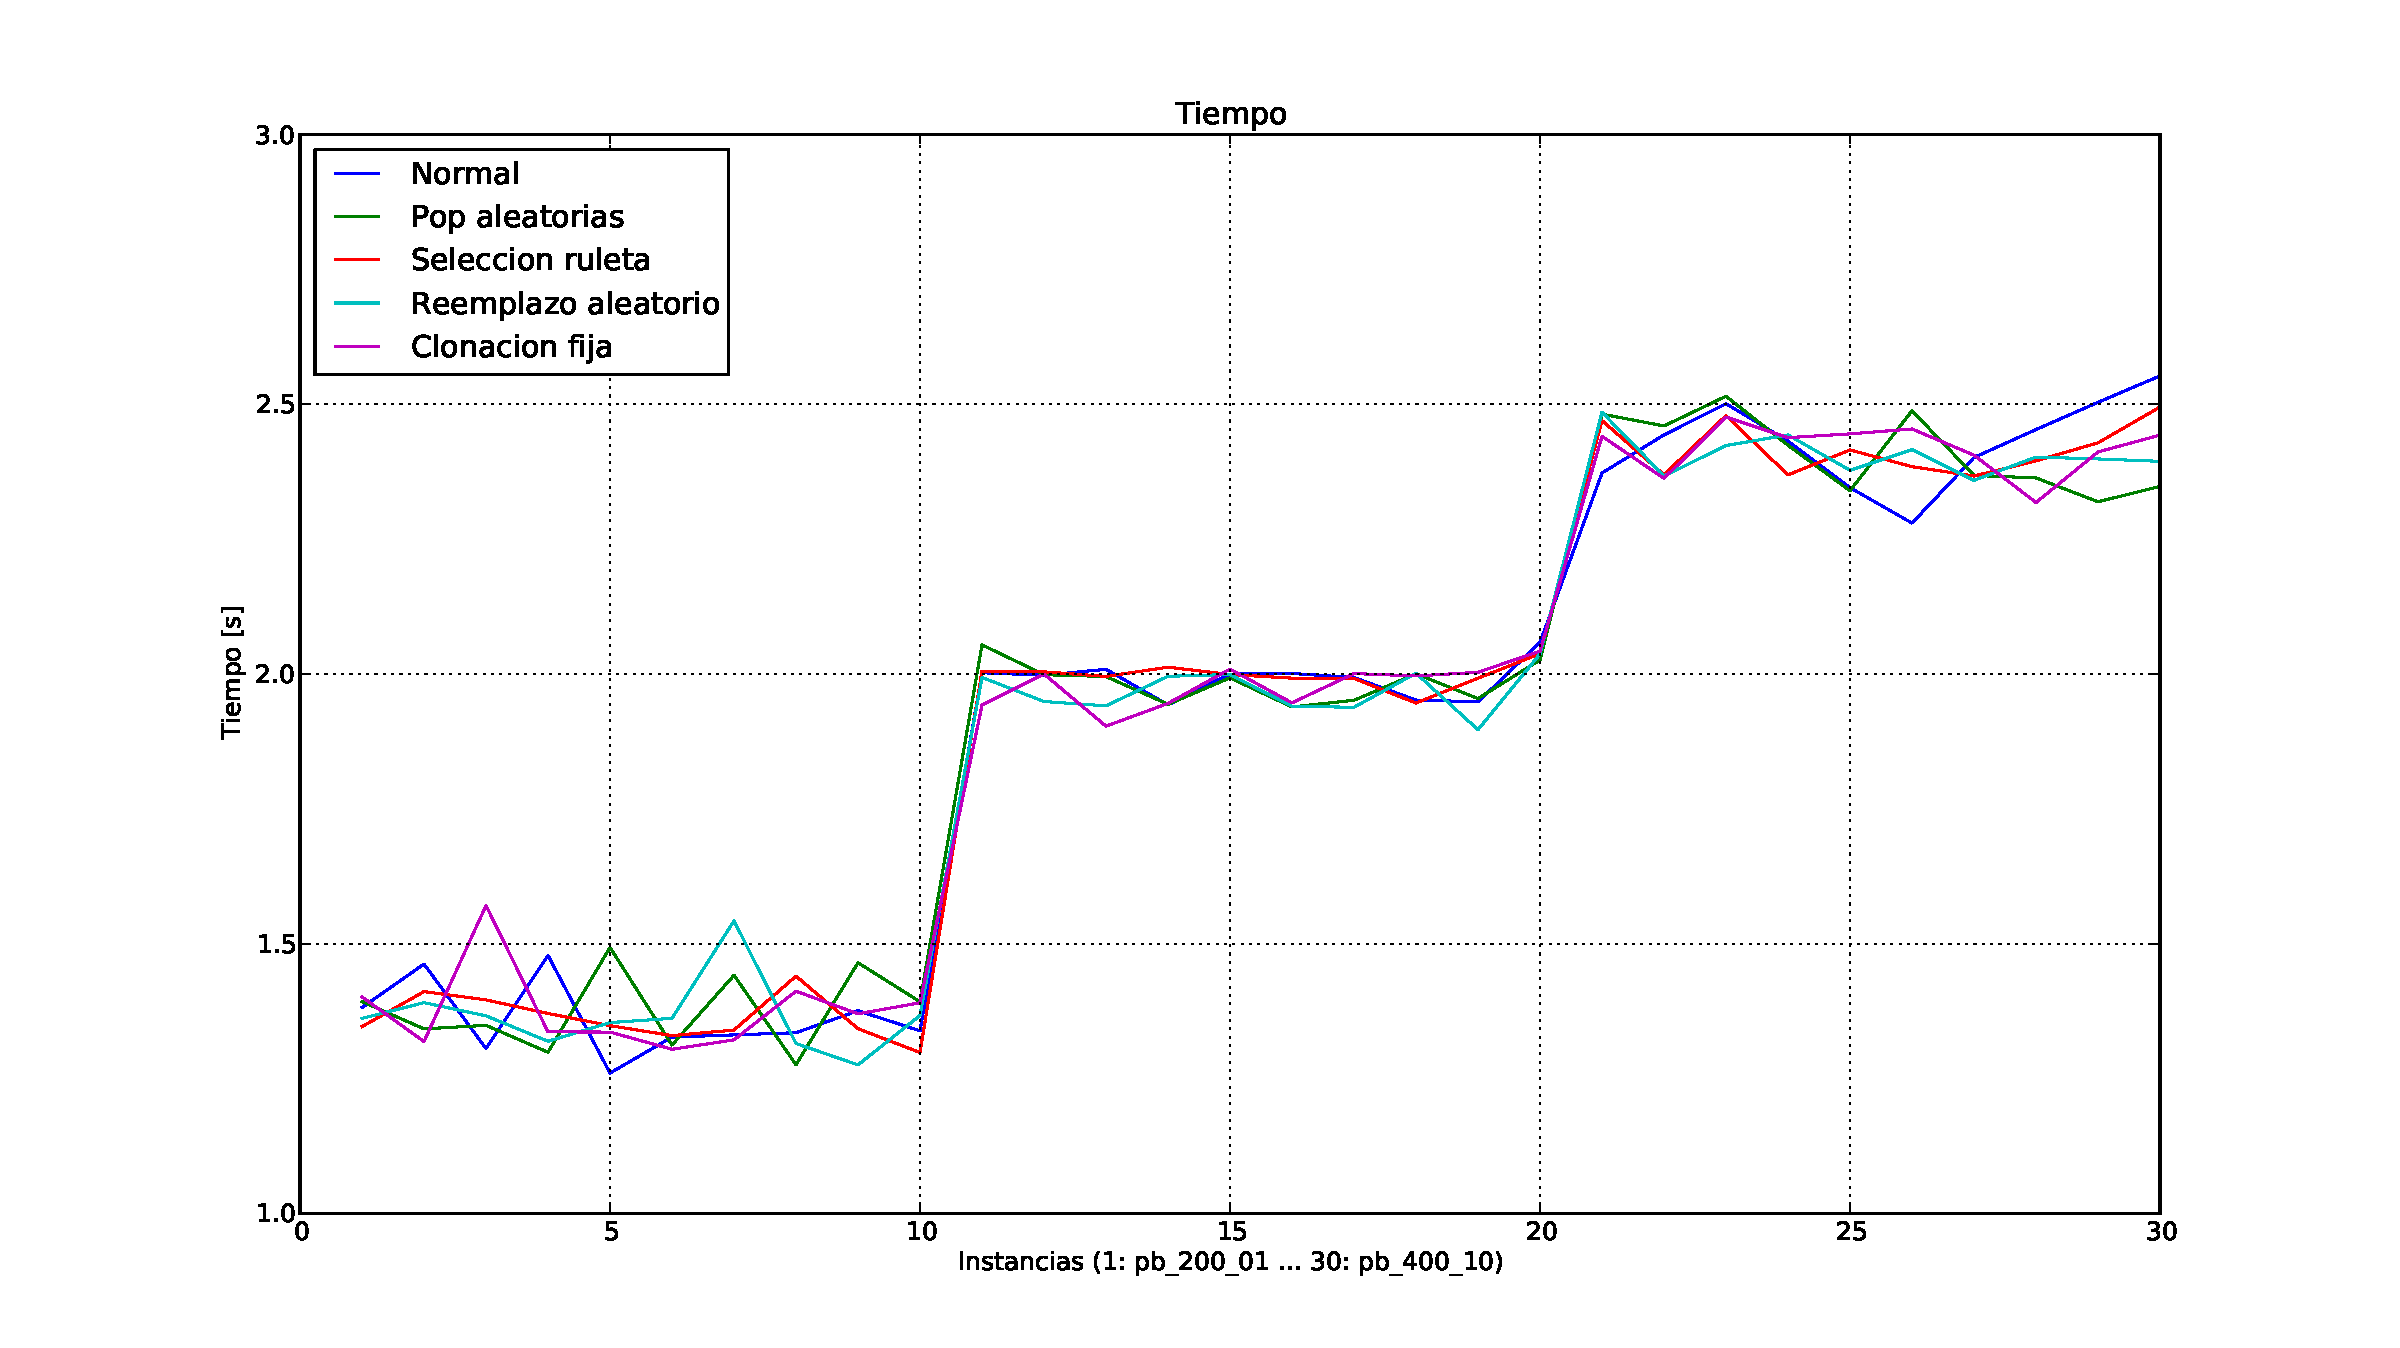
\includegraphics[width=0.95\textwidth]{img/t.pdf}
\end{center}
\caption{Tiempo de ejecución para las modificaciones en cada instancia}
\label{fig:t}
\end{figure}

\begin{figure}[H]
\begin{center}
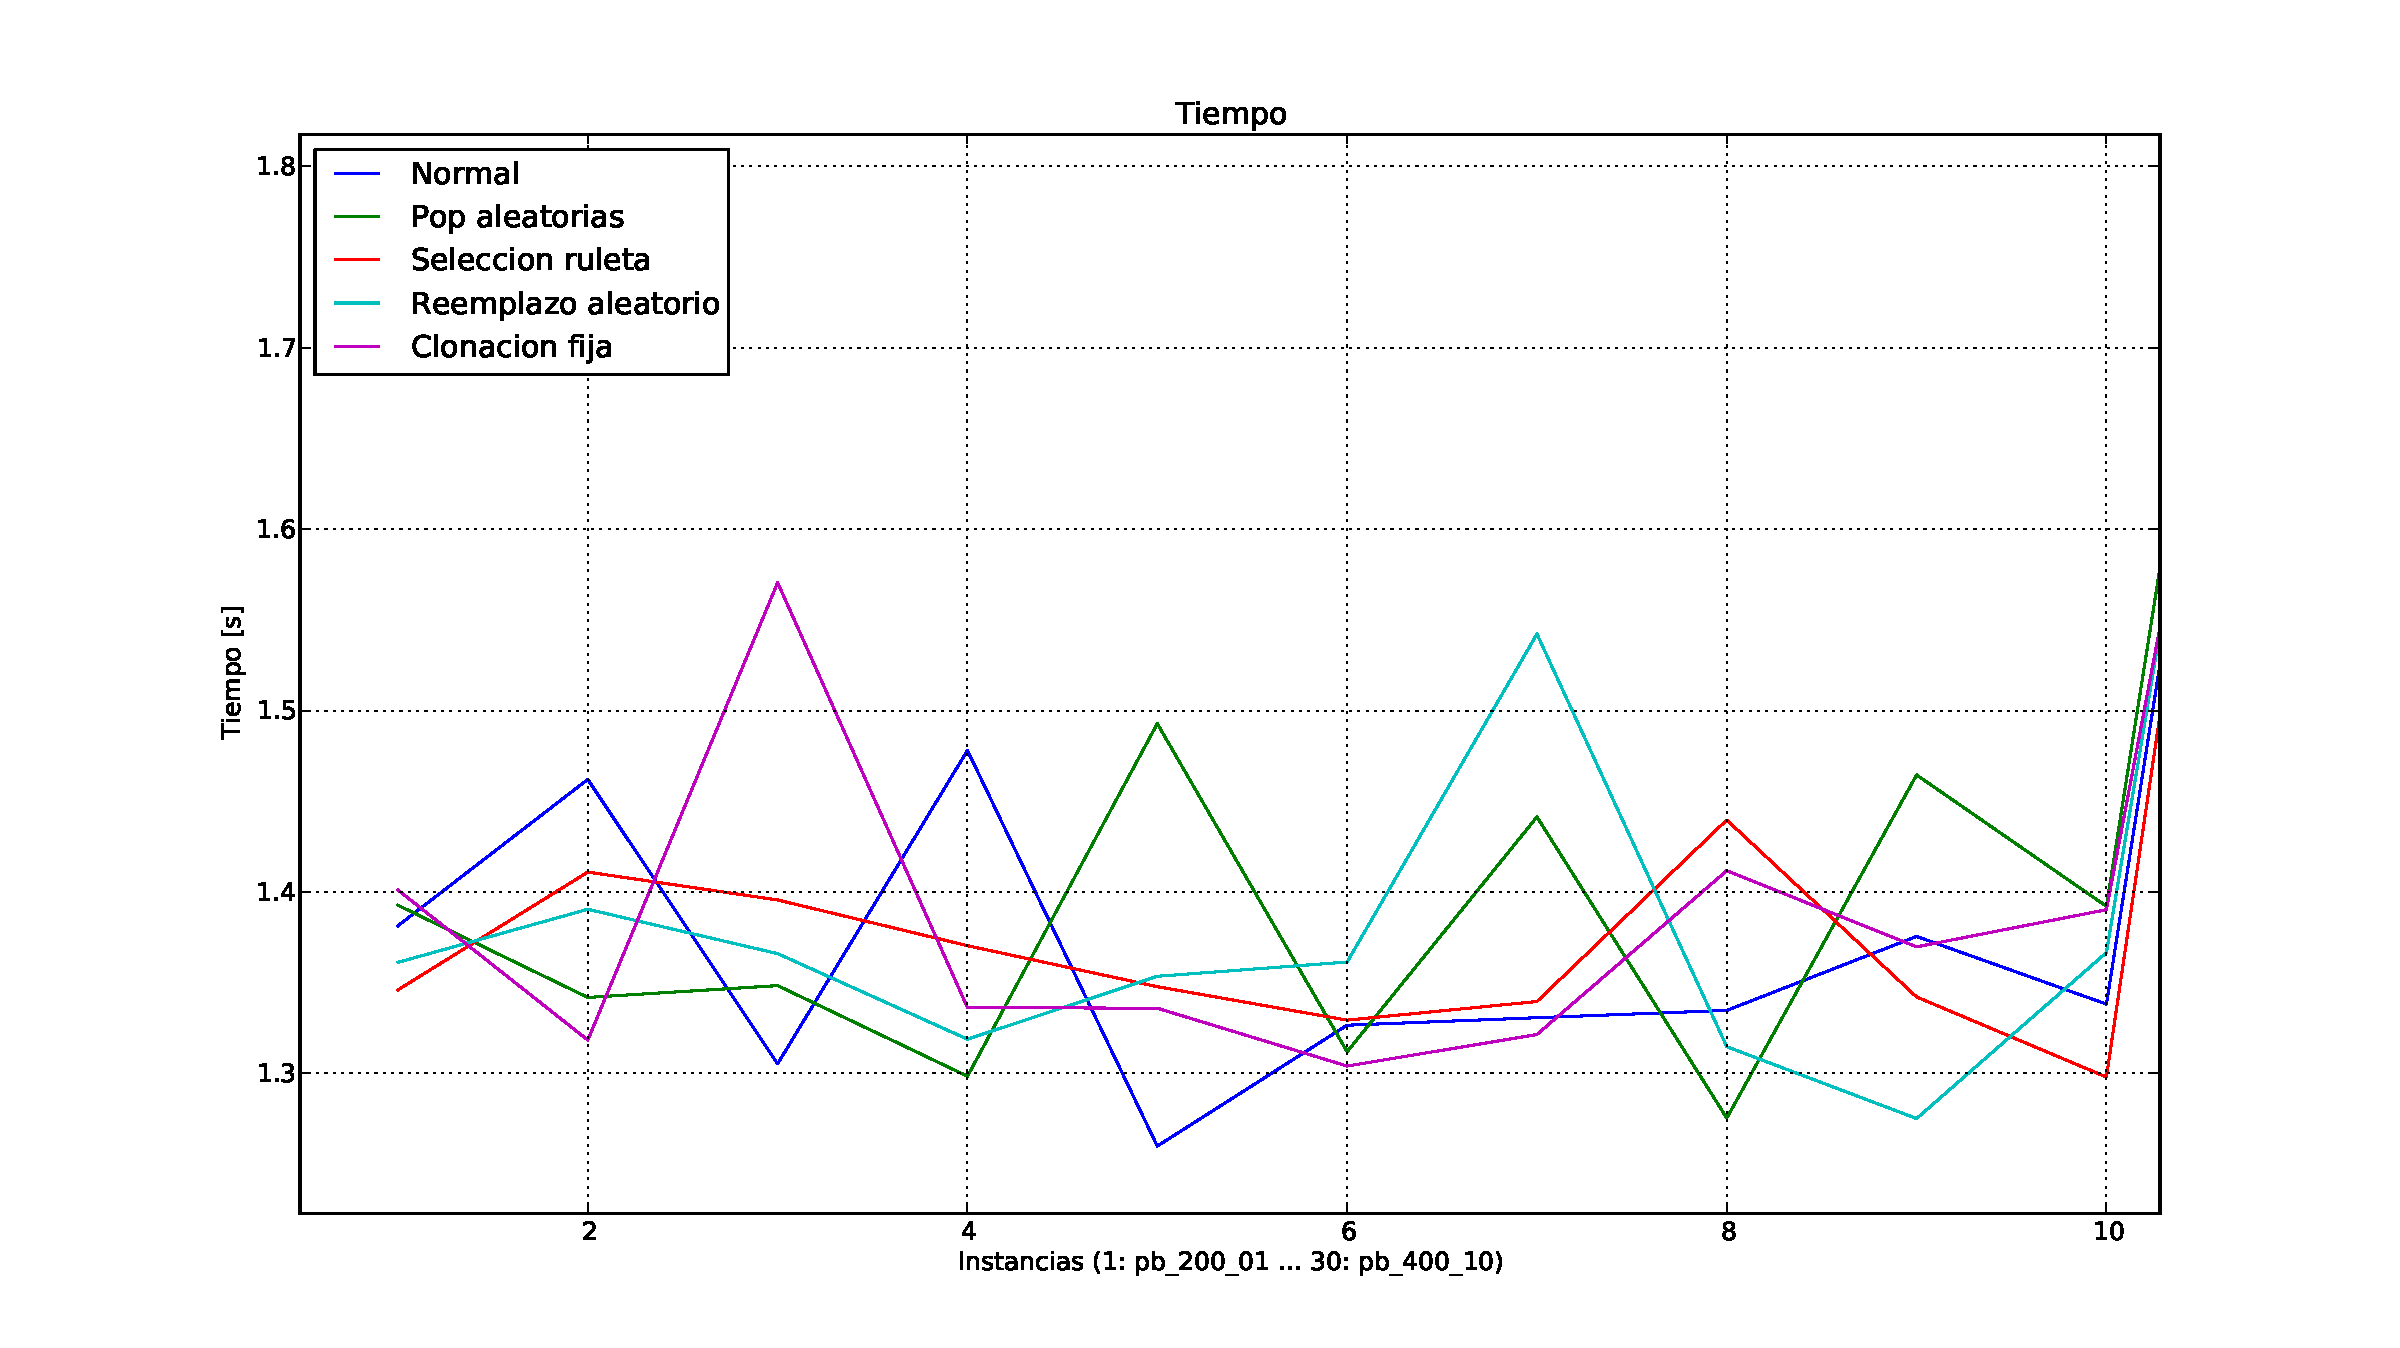
\includegraphics[width=0.95\textwidth]{img/t-zoom200.pdf}
\end{center}
\caption{Tiempo de ejecución para las modificaciones en cada instancia (Zoom a las instancias de 200)}
\label{fig:t200}
\end{figure}

\begin{figure}[H]
\begin{center}
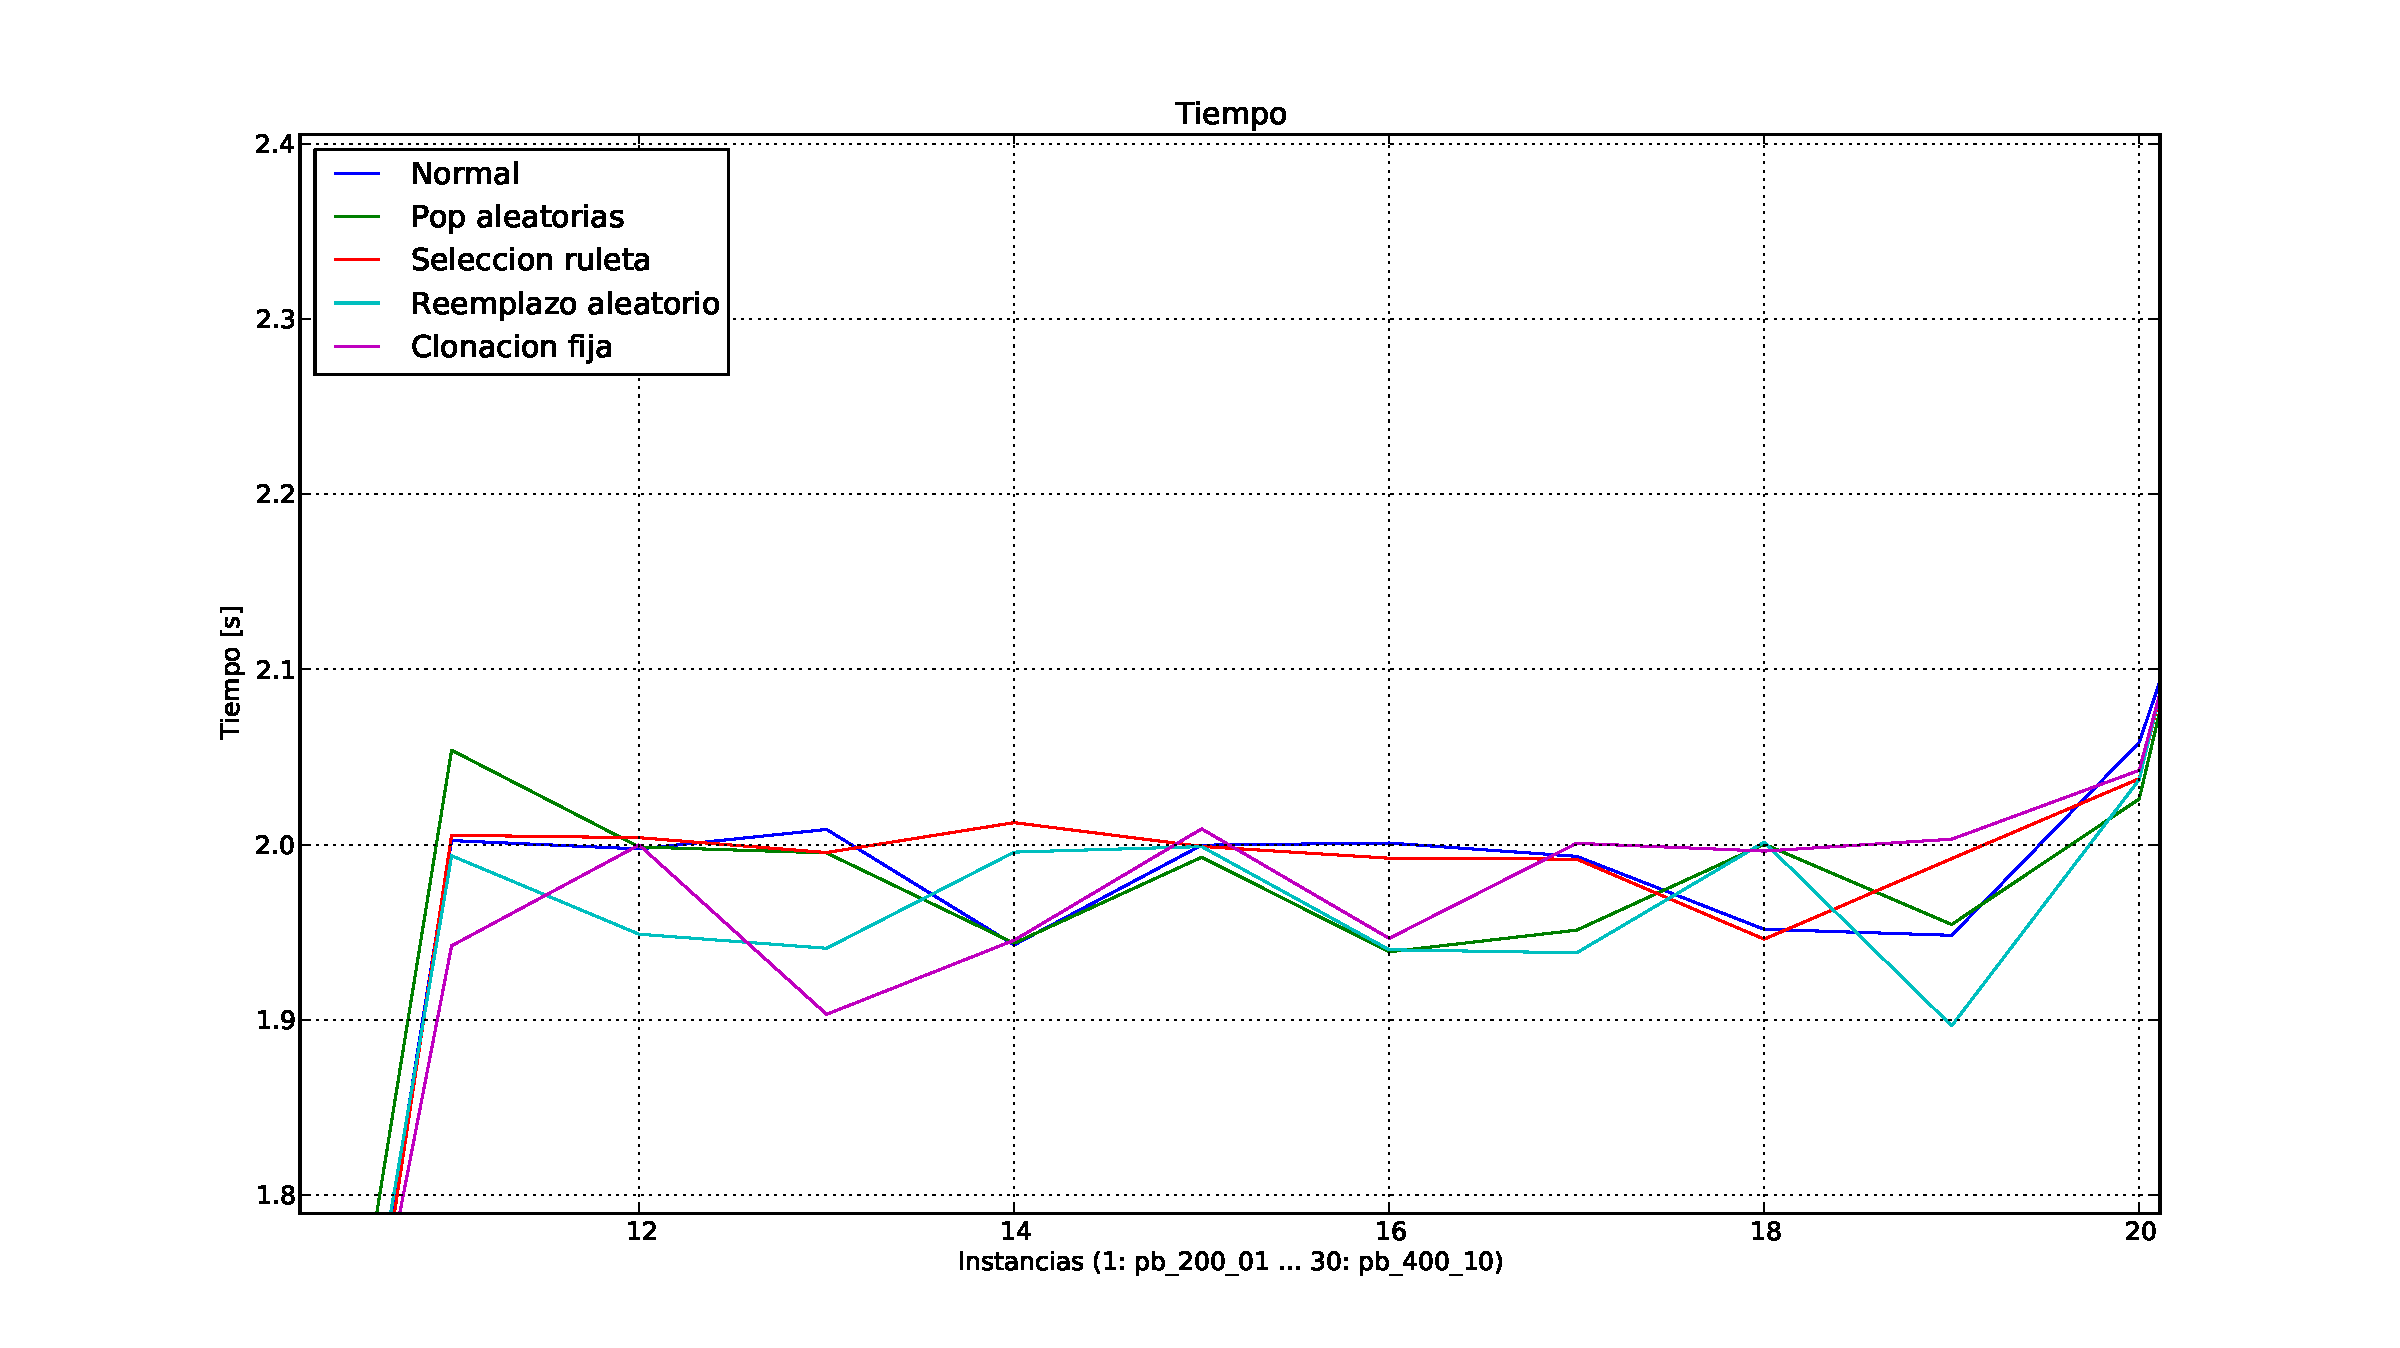
\includegraphics[width=0.95\textwidth]{img/t-zoom300.pdf}
\end{center}
\caption{Tiempo de ejecución para las modificaciones en cada instancia (Zoom a las instancias de 300)}
\label{fig:t300}
\end{figure}

\begin{figure}[H]
\begin{center}
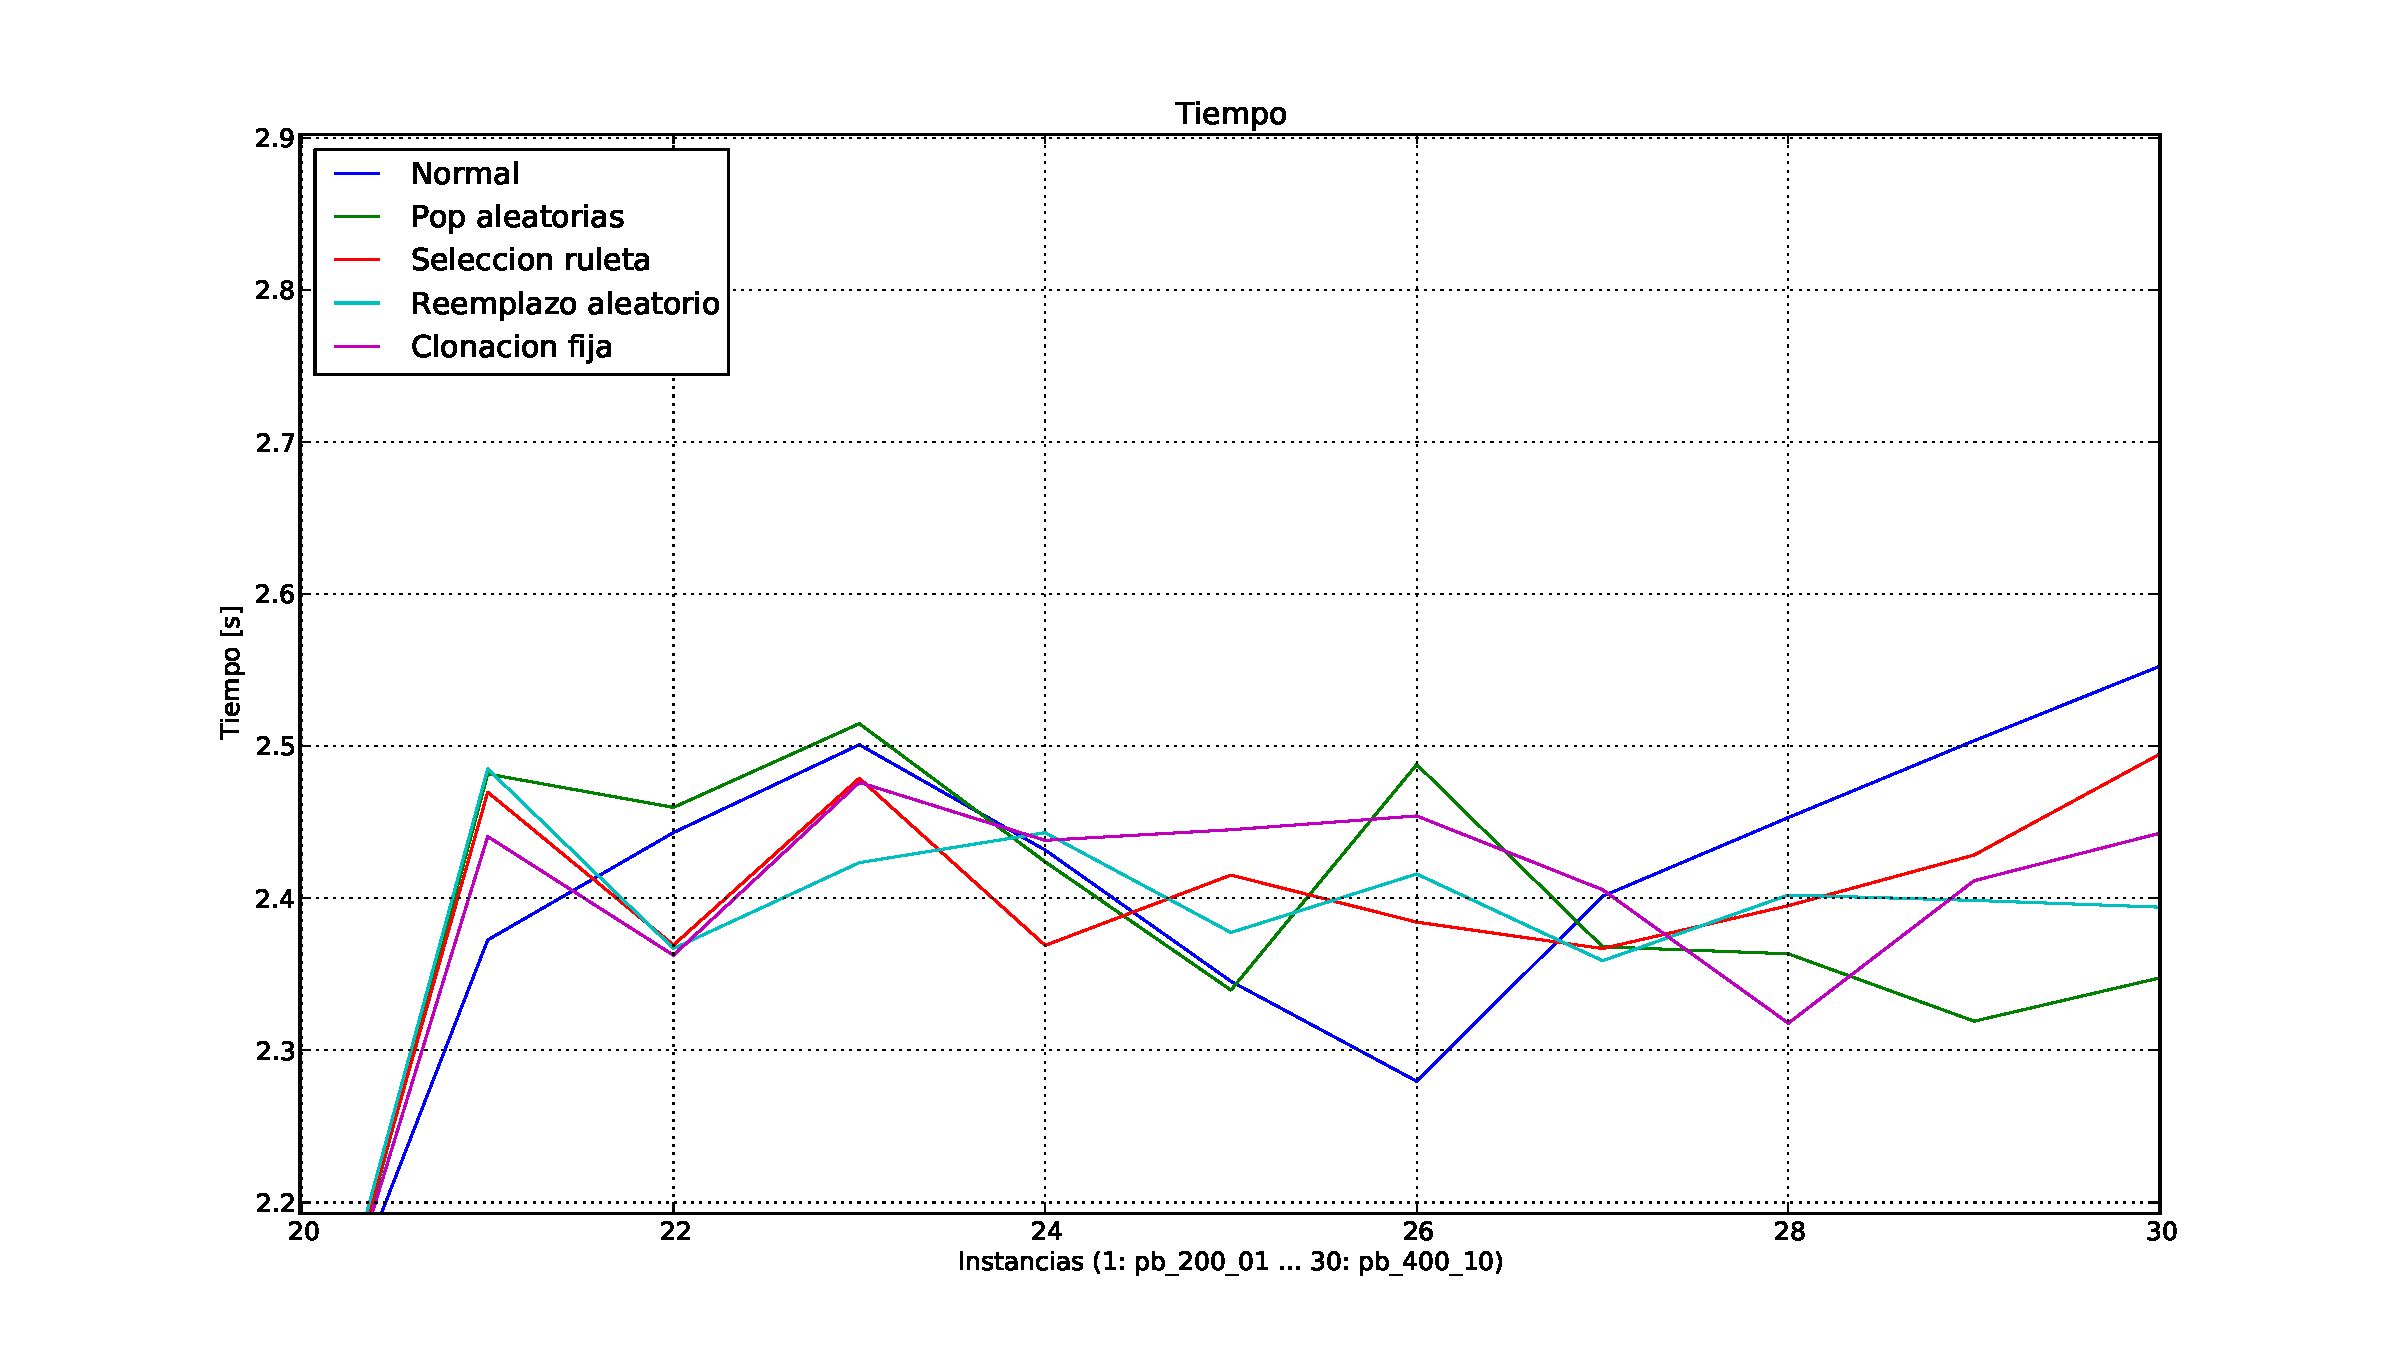
\includegraphics[width=0.95\textwidth]{img/t-zoom400.pdf}
\end{center}
\caption{Tiempo de ejecución para las modificaciones en cada instancia (Zoom a las instancias de 400)}
\label{fig:t400}
\end{figure}
